\documentclass[a4paper,12pt]{article}[abntex2]
\bibliographystyle{abntex2-alf}
\usepackage{siunitx} % Fornece suporte para a tipografia de unidades do Sistema Internacional e formatação de números
\usepackage{booktabs} % Melhora a qualidade das tabelas
\usepackage{tabularx} % Permite tabelas com larguras de colunas ajustáveis
\usepackage{graphicx} % Suporte para inclusão de imagens
\usepackage{newtxtext} % Substitui a fonte padrão pela Times Roman
\usepackage{ragged2e} % Justificação de texto melhorada
\usepackage{setspace} % Controle do espaçamento entre linhas
\usepackage[a4paper, left=3.0cm, top=3.0cm, bottom=2.0cm, right=2.0cm]{geometry} % Personalização das margens do documento
\usepackage{lipsum} % Geração de texto dummy 'Lorem Ipsum'
\usepackage{fancyhdr} % Customização de cabeçalhos e rodapés
\usepackage{titlesec} % Personalização dos títulos de seções
\usepackage[portuguese]{babel} % Adaptação para o português (nomes e hifenização
\usepackage{hyperref} % Suporte a hiperlinks
\usepackage{indentfirst} % Indentação do primeiro parágrafo das seções
\sisetup{
  output-decimal-marker = {,},
  inter-unit-product = \ensuremath{{}\cdot{}},
  per-mode = symbol
}
\DeclareSIUnit{\real}{R\$}
\newcommand{\real}[1]{R\$#1}
\setlength{\headheight}{14.49998pt}
\usepackage{float} % Melhor controle sobre o posicionamento de figuras e tabelas
\usepackage{footnotehyper} % Notas de rodapé clicáveis em combinação com hyperref
\hypersetup{
    colorlinks=true,
    linkcolor=black,
    filecolor=magenta,      
    urlcolor=cyan,
    citecolor=black,        
    pdfborder={0 0 0},
}
\usepackage[normalem]{ulem} % Permite o uso de diferentes tipos de sublinhados sem alterar o \emph{}
\makeatletter
\def\@pdfborder{0 0 0} % Remove a borda dos links
\def\@pdfborderstyle{/S/U/W 1} % Estilo da borda dos links
\makeatother
\onehalfspacing

\begin{document}

\begin{titlepage}
    \centering
    \vspace*{1cm}
    \Large\textbf{INSPER – INSTITUTO DE ENSINO E PESQUISA}\\
    \Large ECONOMIA\\
    \vspace{1.5cm}
    \Large\textbf{Tradução Tópico 9.1 - HPE}\\
    \vspace{1.5cm}
    Prof. Pedro Duarte\\
    Prof. Auxiliar Guilherme Mazer\\
    \vfill
    \normalsize
    Hicham Munir Tayfour, \href{mailto:hichamt@al.insper.edu.br}{hichamt@al.insper.edu.br}\\
    4º Período - Economia B\\
    \vfill
    São Paulo\\
    Abril/2024
\end{titlepage}

\newpage
\tableofcontents
\thispagestyle{empty} % This command removes the page number from the table of contents page
\newpage
\setcounter{page}{1} % This command sets the page number to start from this page
\justify
\onehalfspacing

\pagestyle{fancy}
\fancyhf{}
\rhead{\thepage}

\section{\textbf{Friedman e Schwartz (1966, cap. 13)}}
\subsection{\textbf{Resumo}}

A história monetária dos Estados Unidos durante o século desde a Guerra Civil foi colorida e variada. Ao traçarmos seu percurso tortuoso, achamos necessário explorar a política doméstica, arranjos econômicos internacionais, o funcionamento de grandes organizações administrativas, o papel da personalidade na formação dos eventos e outros assuntos aparentemente distantes da sala de contabilidade. O caráter variado da história monetária dos EUA torna este século de experiência particularmente valioso para o estudante de mudança econômica. Ele não pode controlar o experimento, mas pode observar a experiência monetária sob condições suficientemente distintas para distinguir o que é comum do que é adventício e adquirir considerável confiança de que o que é comum pode ser contado para se manter em outras circunstâncias ainda.

Ao longo do quase século examinado em detalhe, descobrimos que:

1. As mudanças no comportamento do estoque monetário estiveram intimamente associadas a mudanças na atividade econômica, renda monetária e preços.

2. A inter-relação entre mudança monetária e econômica tem sido altamente estável.

3. Mudanças monetárias muitas vezes tiveram uma origem independente; elas não foram simplesmente um reflexo das mudanças na atividade econômica.
Estes elementos comuns da experiência monetária podem ser esperados para caracterizar nosso futuro assim como caracterizaram nosso passado. Além disso, podemos esperar que o futuro, como o passado, forneça mais exemplos da generalização menos específica de que:

4. Em questões monetárias, as aparências enganam; as relações importantes são muitas vezes exatamente o oposto daquelas que parecem óbvias.

\subsubsection{\textbf{Relação Entre o Estoque de Dinheiro e Outras Variáveis Econômicas}}

De 1867 a 1960, nos 93 anos para os quais temos estimativas do estoque de dinheiro, ocorreram duas grandes inflações de preços: um aumento de mais do que o dobro dos preços de 1914 a 1920 e novamente de 1939 a 1948, períodos durante e após cada uma das duas guerras mundiais. Em ambas as guerras, houve também mais do que uma duplicação no estoque de dinheiro. Um aumento tão grande no estoque de dinheiro em um tempo correspondentemente breve não ocorreu em nenhum outro período.

Um aumento substancial e relativamente prolongado dos preços em tempos de paz ocorreu apenas em um período: de 1897 a 1914, quando os preços aumentaram de 40 a 50 por cento. A taxa média anual de aumento do estoque de dinheiro de 1897 a 1914 foi maior do que durante qualquer outro período de comprimento comparável que exclui as duas guerras mundiais. Temia-se amplamente que o período pós-Segunda Guerra Mundial pudesse acabar sendo outro período de aumento prolongado nos preços. No entanto, até 1960, claramente não era o caso. Os principais aumentos de preços desde 1945 foram ou uma continuação da Segunda Guerra Mundial ou relacionados à Guerra da Coreia.

Caracterizamos quatro segmentos dos 93 anos como apresentando um grau relativamente alto de estabilidade econômica: 1882-92, 1903-13, 1923-29, 1948-60. Cada um também exibiu um alto grau de estabilidade da mudança de ano para ano no estoque de dinheiro; os períodos restantes mostraram uma instabilidade consideravelmente maior da mudança de ano para ano tanto no dinheiro quanto na renda.

Em 93 anos, houve seis períodos de contração econômica severa que produziram angústia generalizada e desemprego. Historiadores de ciclos econômicos classificam essas contrações como de uma ordem de magnitude diferente, senão de uma espécie diferente das contrações mais leves que ocorreram, em média, a cada quatro anos (ver Gráfico 62). A contração mais severa foi de 1929 a 1933. As outras foram 1873-79, 1893-94 — ou melhor, talvez, todo o período de 1893 a 1897, que continha duas contrações de ciclo de negócios separadas por uma breve e incompleta expansão — 1907-08, 1920-21 e 1937-38. Cada uma dessas contrações severas foi acompanhada por uma queda apreciável no estoque de dinheiro, sendo a queda mais severa durante a contração de 1929-33. A única outra queda comparável em magnitude às seis foi no primeiro ano da série, de 1867 a 1868, o estágio final da liquidação de alguns expedientes monetários da Guerra Civil. Houve apenas outros dois períodos nos 93 anos inteiros em que o estoque de dinheiro diminuiu apreciavelmente por mais do que alguns meses isolados, 1948-49 e 1959-60, e as quedas nesses períodos foram decididamente menores em magnitude do que em qualquer uma das seis contrações severas. As contrações restantes deixaram sua marca na forma de uma taxa de crescimento mais lenta do estoque de dinheiro durante as contrações do que durante as expansões, em vez de uma queda absoluta.

Das seis contrações severas, quatro foram caracterizadas por grandes perturbações bancárias ou monetárias: 1873-79, marcado pela controvérsia sobre os "greenbacks" e a retomada dos pagamentos em espécie, além de uma crise bancária em 1873; a década de 1890, pela controvérsia sobre o papel da prata, uma crise bancária em 1890 e uma crise bancária mais severa em 1893 envolvendo uma restrição concertada pelos bancos na conversibilidade de depósitos em moeda; 1907-08, por um pânico bancário que também envolveu restrição; e 1929-33, pelo colapso do sistema bancário que resultou no desaparecimento por falência ou fusão de um terço dos bancos e terminou em um feriado bancário nacional e na cessação completa das atividades bancárias por uma semana. Apenas uma outra crise bancária comparável em gravidade às quatro ocorreu durante todo o período: a crise bancária de 1884, um episódio no decorrer da terceira maior contração do nosso período (1882 a 1885), que está no limite para inclusão em nossa lista de contrações severas.

Nas outras duas contrações severas, 1920-21 e 1937-38, o declínio no estoque de dinheiro foi consequência de ações políticas do Sistema da Reserva Federal: em 1920-21, um aumento acentuado na taxa de desconto no início de 1920 seguido por outro aumento semelhante cerca de quatro meses e meio depois; em 1937-38, uma duplicação dos requisitos de reserva em 1936 e início de 1937. Em ambos os casos, o declínio subsequente no estoque de dinheiro foi associado a um grave declínio econômico, mas em nenhum dos casos levou a uma crise bancária.

Das relações reveladas por nossa evidência, as mais próximas são entre, por um lado, movimentos seculares e cíclicos no estoque de dinheiro e, por outro, movimentos correspondentes na renda monetária e preços. Como a renda real tende a variar ao longo do ciclo na mesma direção que a renda monetária, também observamos uma relação próxima entre os movimentos cíclicos no estoque de dinheiro e na renda real ou atividade empresarial. A relação entre movimentos seculares no estoque de dinheiro e na renda real é muito menos próxima. A renda real cresceu a taxas praticamente iguais durante cada um dos quatro períodos de estabilidade listados anteriormente. No entanto, o estoque de dinheiro e os preços cresceram a taxas bastante diferentes, com preços declinando 1 por cento ao ano em um período e subindo 2 por cento ao ano em outro. Aparentemente, as forças que determinam a taxa de crescimento de longo prazo da renda real são em grande parte independentes da taxa de crescimento de longo prazo do estoque de dinheiro, contanto que ambos prossigam de maneira bastante uniforme. Mas a instabilidade marcada do dinheiro é acompanhada por instabilidade do crescimento econômico.

\begin{figure}[H]
    \centering
    \caption{Gráfico 62}
    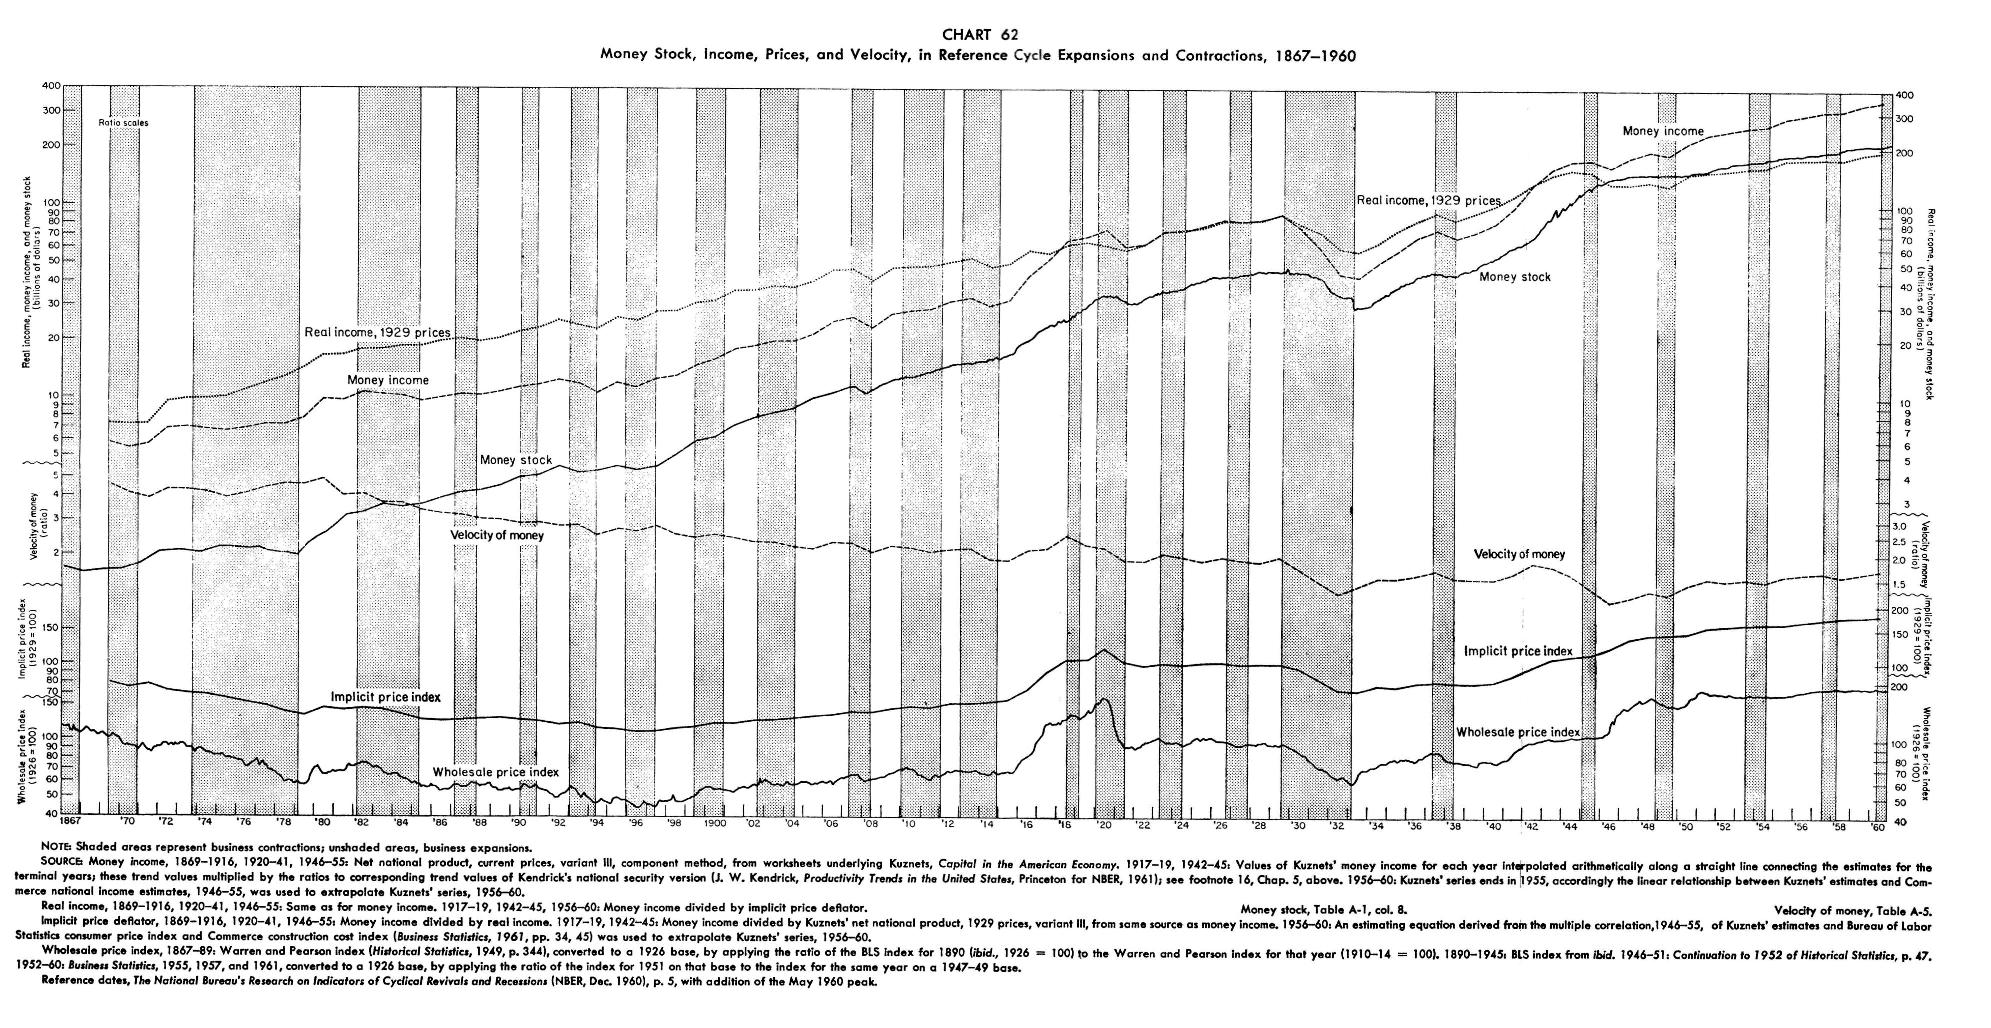
\includegraphics[width=1.0\textwidth]{4º Período/História do Pensamento Econômico/Tradução HPE/Tradução Tópico 9.1/Gráfico 62.png}
    \end{figure}
    
\subsubsection{\textbf{Estabilidade das Relações Monetárias}}

A relação entre dinheiro e outras variáveis econômicas não só tem sido próxima, mas também altamente estável em forma e caráter. Um exemplo marcante da estabilidade das relações econômicas básicas é o comportamento dos preços relativos nos Estados Unidos e na Grã-Bretanha, ajustados pelas mudanças na taxa de câmbio entre o dólar e a libra. Temos uma série razoavelmente contínua desde 1871 (Gráfico 63). Nos 79 anos de 1871 a 1949, ocorreram vastas mudanças na estrutura econômica e no desenvolvimento dos Estados Unidos, no papel da Grã-Bretanha na economia mundial, nas estruturas monetárias internas de ambos os países e nos arranjos monetários internacionais que os ligavam. No entanto, apesar dessas mudanças, apesar de duas guerras mundiais e apesar dos erros estatísticos nos números dos índices de preços, a razão de preço ajustada, expressa em uma base que faz 1929 = 100, esteve entre 84 e 111 em todos, exceto um dos 79 anos. A exceção foi 1932. Refletiu a desordem das relações monetárias internacionais que se seguiu à desvalorização da Grã-Bretanha no outono de 1931, que tornou a Grã-Bretanha temporariamente não representativa do mundo fora da área da libra com a qual os Estados Unidos negociavam. Dentro de um ano, a razão voltou ao intervalo anterior. Além disso, quase os extremos do intervalo foram experimentados na própria primeira década, durante a qual a razão variou de 111 em 1871 a 86 em 1876. Em 1950, depois que a Grã-Bretanha desvalorizou novamente no outono de 1949, a razão, como em 1932, disparou para fora do intervalo anterior, desta vez por uma quantidade muito mais significativa, para 143. Essa divergência durou mais tempo, em parte devido ao papel menor que a Grã-Bretanha passou a desempenhar na economia mundial, mas ainda mais, acreditamos, devido ao desenvolvimento de técnicas mais eficazes para suprimir a expressão de aumentos de preços ou seu equivalente em números de índices de preços computados. No entanto, ano a ano, a razão declinou até 1958, quando atingiu 118, apenas ligeiramente fora do intervalo anterior; e permaneceu aproximadamente nesse nível até 1960.

Mesmo que estejamos acostumados a considerar os Estados Unidos como quase autossuficientes, a integração econômica do mundo ocidental tem sido suficientemente próxima para deixar os preços dos EUA com pouca margem de manobra em relação aos preços externos, quando ambos são expressos em uma moeda comum. Houve mais flexibilidade em como a relação de preços foi alcançada — seja por meio de mudanças nos preços internos ou nas taxas de câmbio — do que na relação que poderia ser alcançada. Variações amplas em tarifas, um grande programa de compra de ouro, mudanças vastas na direção dos movimentos de capital (veja Gráfico 63) ou a imposição por nossos parceiros comerciais de controles extensivos de câmbio — nenhum desses fatores alterou radicalmente as relações de preços necessárias para produzir alguma medida de equilíbrio nos pagamentos internacionais.

\begin{figure}[H]
    \centering
    \caption{Gráfico 63}
    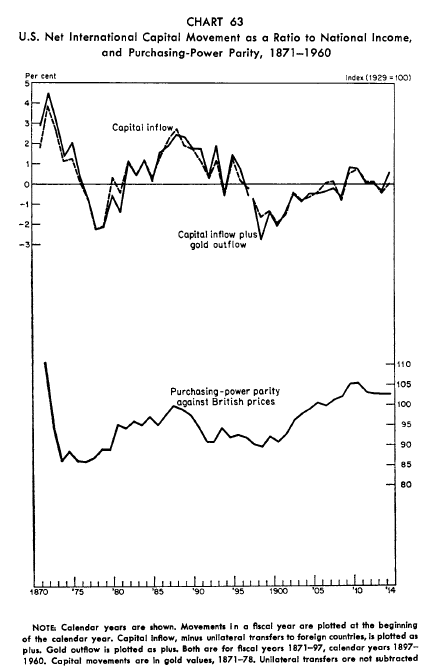
\includegraphics[width=1.0\textwidth]{4º Período/História do Pensamento Econômico/Tradução HPE/Tradução Tópico 9.1/Gráfico 63.png}
    \end{figure}

\begin{figure}[H]
    \centering
    \caption{Gráfico 63(Concluido)}
    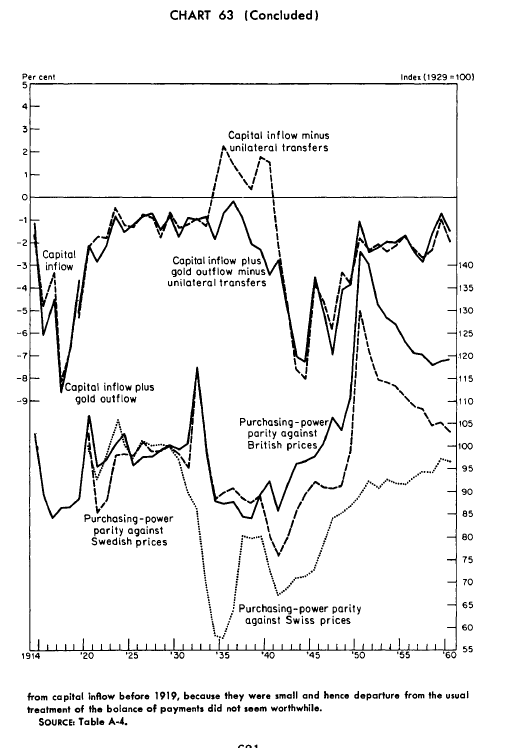
\includegraphics[width=1.0\textwidth]{4º Período/História do Pensamento Econômico/Tradução HPE/Tradução Tópico 9.1/Gráfico 63(Concluido).png}
    \end{figure}

A velocidade do dinheiro, que reflete as propensões de retenção de dinheiro da comunidade, oferece outro exemplo da estabilidade das relações monetárias básicas. À medida que a renda real da população dos Estados Unidos aumentava, e talvez também à medida que os depósitos se tornavam mais convenientes com a expansão das facilidades bancárias, a comunidade passou a reter uma quantidade consideravelmente maior de dinheiro em relação à sua renda, o que significa que a velocidade do dinheiro diminuiu. Em 1869, o estoque de dinheiro correspondia a menos de três meses de renda; em 1960, a mais de sete meses de renda. O valor numérico da velocidade, portanto, mudou consideravelmente. No entanto, a mudança ocorreu de forma bastante estável: um pouco mais rapidamente quando os preços estavam caindo durante a década de 1880 e início dos anos 1890, tornando a retenção de dinheiro mais atraente; e um pouco mais lentamente quando os preços estavam subindo de 1897 a 1914. As únicas grandes exceções foram durante e após a grande contração dos anos 1930, que viu uma grande queda na velocidade seguida de uma recuperação, e durante e após a Segunda Guerra Mundial, que também viu uma grande queda na velocidade seguida de uma recuperação pós-guerra. Em resposta às flutuações cíclicas, a velocidade mostrou um movimento sistemático e estável em torno de sua tendência, aumentando durante a expansão e diminuindo durante a contração. Mesmo o grande movimento que acompanhou a Grande Contração se encaixa parcialmente neste padrão; foi tão grande em parte porque o movimento cíclico foi muito grande.

Durante as nove décadas que terminaram em 1960, a velocidade do dinheiro caiu em média pouco mais de 1 por cento ao ano. Durante expansões econômicas, ela subiu ou caiu a uma taxa menor que essa; durante contrações, ela diminuiu a uma taxa maior que essa. As amplitudes do aumento e queda cíclicos tendiam a variar com a amplitude dos movimentos cíclicos na atividade econômica. Como muitos dos movimentos cíclicos na atividade econômica tinham aproximadamente a mesma amplitude, muitos dos movimentos cíclicos na velocidade também a tinham. Apesar da tendência secular, do padrão cíclico consistente e da margem de erro considerável em nossas estimativas, a mudança observada de ano para ano na velocidade foi inferior a 10 por cento em 78 das 91 mudanças de ano para ano de 1869, quando nossas figuras de velocidade começam, até 1960. Das 13 mudanças maiores, mais da metade ocorreu durante a Grande Contração ou as duas guerras mundiais, e a maior mudança foi de 17 por cento. Expressa como uma porcentagem de uma tendência secular, a velocidade estava dentro do intervalo de 90 a 110 em 53 anos, e de 85 a 115 em 66 anos. Dos 26 anos restantes, 12 foram durante os primeiros 15 anos, para os quais os números de renda são seriamente defeituosos, e 7 durante a Grande Contração e as duas guerras mundiais.

Outra relação monetária que tem sido altamente estável é a relação entre as mudanças no estoque de dinheiro e os movimentos cíclicos na atividade econômica. Em média, o estoque de dinheiro cresceu a uma taxa mais alta que a renda monetária; isso é o outro lado da queda secular na velocidade. O aumento foi mais rápido que o usual durante expansões cíclicas e menos rápido que o usual durante contrações cíclicas. A taxa de crescimento tendia a desacelerar bem antes do pico nos negócios e a acelerar bem antes do ponto mais baixo. Esse padrão prevalece durante todo o período, no ciclo mais antigo coberto por nossos dados e também no mais recente.

O leitor atento de nossa narrativa terá encontrado muitos outros exemplos detalhados de relações monetárias estáveis para complementar essas muito amplas: os efeitos semelhantes dos programas de compra de ouro empreendidos em 1878 para preparar a retomada e após 1933 para elevar os preços domésticos; a confiabilidade da razão depósito-moeda como um sinal de um problema de liquidez; os movimentos iniciais semelhantes dos preços no atacado dos EUA após o início das Guerras Mundiais I e II—em ambos os casos, em uma direção oposta à que prevaleceu mais tarde; e assim por diante.

Essas uniformidades persistiram apesar das mudanças radicais nos arranjos monetários. De 1862 a 1879, os Estados Unidos tinham uma moeda nacional independente, não conversível em ouro nem prata nem na moeda de nenhum outro país em qualquer proporção fixa. O estoque de dinheiro poderia, portanto, ser determinado internamente. De 1879 a 1914, o dinheiro dos EUA era conversível em ouro em uma proporção fixa especificada por lei e mantida na prática. O estoque de dinheiro e os preços internos tinham que estar em níveis que produzissem um equilíbrio aproximado nos pagamentos internacionais sem movimentos anormais de ouro. O estoque de dinheiro era uma variável dependente, não independente, embora, é claro, houvesse alguma margem de manobra em períodos curtos. Tanto antes quanto depois de 1879, até que o Sistema da Reserva fosse estabelecido, o sistema bancário unitário dos EUA era dividido entre bancos nacionais e não nacionais, cada um com cerca de metade dos depósitos totais, e nenhum sujeito a qualquer controle central exceto quando o Tesouro de tempos em tempos assumia funções de banco central.

De 1914 a 1933, o dinheiro dos EUA continuou a ser rigidamente vinculado ao ouro, mas o número de outras moedas nacionais assim vinculadas havia diminuído. Os Estados Unidos haviam alcançado um papel muito mais importante na economia mundial, e o comércio externo havia se tornado uma parte menor da atividade econômica dos EUA. Os vínculos entre o dinheiro dos EUA e o comércio internacional, portanto, eram muito mais frouxos do que nos anos anteriores. Além disso, o Federal Reserve Act não apenas estabeleceu controle central sobre a maior parte do sistema bancário, mas também forneceu uma agência que poderia intervir deliberadamente para alterar ou até reverter a relação entre os pagamentos internacionais e o estoque doméstico de dinheiro.

No início de 1933, o vínculo rígido entre o dinheiro dos EUA e o ouro foi rompido. Um ano depois, um vínculo rígido foi restabelecido em uma proporção diferente. No entanto, o padrão-ouro então restabelecido e legalmente vigente desde então era muito diferente do padrão pré-1933. O ouro foi eliminado da circulação, e a posse de ouro monetário por cidadãos privados foi tornada ilegal, de modo que o dinheiro nacional não era mais livremente conversível em ouro em uma proporção fixa. O afrouxamento dos vínculos entre o dinheiro e o ouro e, consequentemente, entre o dinheiro e o comércio internacional foi completado por outros países, muitos dos quais foram ainda mais longe ao cortar toda conexão entre o dinheiro nacional e o ouro. Hoje, o ouro é principalmente uma mercadoria cujo preço é fixado em vez de ser a pedra angular do sistema monetário mundial ou dos EUA. No entanto, o legado da história e o uso do ouro como veículo para fixação das taxas de câmbio ainda lhe conferem uma significância monetária que nenhuma outra mercadoria sujeita à fixação de preços pelo governo possui.

Uma grande mudança ocorreu no sistema bancário em 1934 como resultado do início do seguro federal de depósitos bancários. Parece ter tido sucesso, ao contrário do que ocorreu com o Federal Reserve Act, em tornar impossível a proliferação de uma perda de confiança pública em alguns bancos em um pânico bancário decorrente de uma tentativa generalizada por parte do público de converter depósitos em moeda.

Essas mudanças nos arranjos monetários alteraram significativamente as forças que determinam o estoque de dinheiro. Como resultado, elas também alteraram o comportamento do estoque de dinheiro. Por exemplo, nos 46 anos de 1914 a 1960, quando uma agência governamental tinha responsabilidade explícita pelo comportamento do estoque de dinheiro, a mudança de ano para ano no estoque foi uma magnitude mais variável do que nos 35 anos anteriores, quando era determinada pelo mecanismo quase automático do padrão-ouro. Por outro lado, no período desde o final da Segunda Guerra Mundial, tem sido uma magnitude muito menos variável do que em qualquer período anterior de comprimento comparável (Tabela 25).

As mudanças nos arranjos monetários afetaram de diversas maneiras as três variáveis que consideramos úteis para considerar como os determinantes aritméticos do estoque de dinheiro: o estoque de dinheiro de alta potência; a razão entre os depósitos do público e seus estoques de moeda; e a razão entre as obrigações de depósito do sistema bancário comercial e suas reservas, que definimos como igual aos seus totais de dinheiro de alta potência (Gráfico 64).

O estoque de dinheiro de alta potência foi o principal fator que contabilizou aritmeticamente as mudanças no estoque de dinheiro. As mudanças no dinheiro de alta potência, no entanto, foram produzidas por diferentes forças em diferentes momentos: no período dos "greenbacks", principalmente por mudanças nas emissões fiduciárias do governo; de 1879 a 1914, principalmente por fluxos de ouro, embora em alguma medida também por mudanças em notas bancárias nacionais e moeda emitida em troca de prata; de 1914 a 1960, principalmente por mudanças no crédito em circulação do Federal Reserve, com a notável exceção dos anos de 1934 a 1940, quando os fluxos de ouro dominaram.

\begin{figure}[H]
    \centering
    \caption{Gráfico 64}
    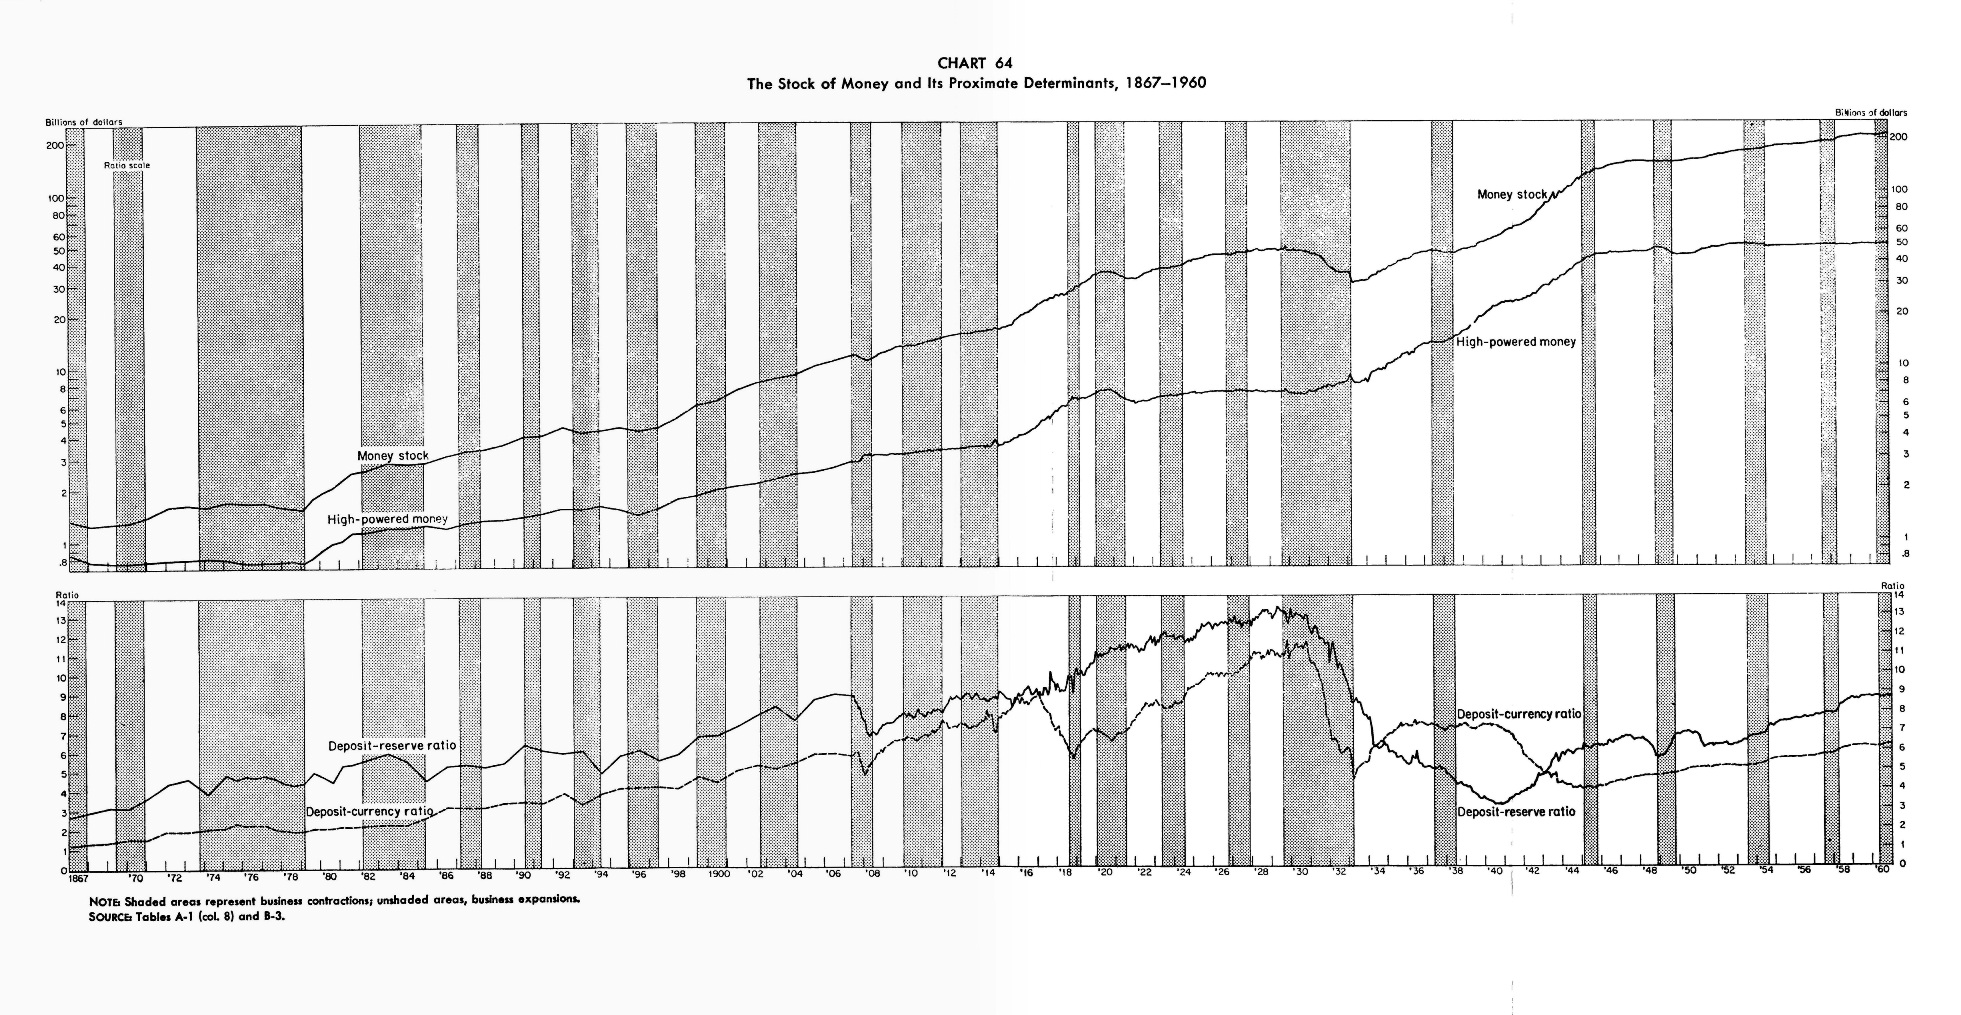
\includegraphics[width=1.0\textwidth]{4º Período/História do Pensamento Econômico/Tradução HPE/Tradução Tópico 9.1/Gráfico 64.png}
    \end{figure}

A relação depósito-moeda tem sido de grande importância principalmente durante períodos de dificuldades financeiras. Em cada um desses períodos, a perda de confiança do público nos bancos levou a uma tentativa de converter depósitos em moeda, o que resultou em uma forte queda na relação depósitos-moeda e uma forte pressão descendente sobre o estoque de dinheiro. Esperava-se que a criação do Sistema da Reserva Federal privasse tais mudanças na relação depósito-moeda de significância monetária, fornecendo um meio de aumentar o volume absoluto de moeda disponível para o público segurar, quando o público desejasse substituir depósitos por moeda, sem exigir uma contração múltipla dos depósitos. Na prática, isso não conseguiu alcançar esse objetivo. A mudança mais notável na relação depósito-moeda nos 93 anos de 1867 a 1960 ocorreu de 1930 a 1933, quando a relação caiu para menos da metade de seu valor inicial e, em três anos, apagou o aumento secular de três décadas. Embora o volume absoluto de moeda mantido pelo público tenha aumentado, isso ocorreu apenas à custa de uma queda muito maior nos depósitos, o efeito combinado sendo uma queda de um terço no estoque total de dinheiro. O início do seguro federal de depósitos bancários em 1934 finalmente mudou decisivamente o comportamento da relação depósito-moeda. Desde então, não tem sido sujeita a mudanças drásticas em curtos períodos, e é improvável que seja no futuro.

A relação depósitos-reservas, assim como a relação depósito-moeda, tem sido de grande importância em tempos de dificuldades financeiras, embora tenha desempenhado um papel mais consistente e menor, geralmente aumentando durante expansões empresariais e caindo durante contrações empresariais. Sempre que o público demonstrou desconfiança dos bancos ao procurar reduzir a relação depósito-moeda, os bancos reagiram procurando fortalecer suas reservas. Após um breve intervalo, eles conseguiram fazer isso, ou seja, baixando a relação depósito-reserva, adicionando assim mais pressão descendente sobre o estoque de dinheiro.

A relação depósito-reserva também variou ao longo de períodos mais longos em resposta a mudanças nos arranjos monetários. Aumentou notavelmente no período dos greenbacks como resultado da maturação dos bancos nacionais e um aumento na importância relativa dos bancos não nacionais. Aumentou novamente na década de 1897 a 1907, em parte como resultado da assunção pelo Tesouro de funções bancárias centrais mais amplas. Aumentou novamente após o estabelecimento do Sistema da Reserva Federal, que reduziu os requisitos legais e deu aos bancos a confiança de que, em caso de necessidade, eles tinham um "emprestador de última instância" para recorrer. O colapso monetário de 1930 a 1933 mudou profundamente o cenário. Produziu uma queda na relação depósito-reserva de seu ponto mais alto em 1929 para um nível, uma década depois, não muito acima do nível no início da nossa série em 1867. A experiência de 1930-33 ensinou aos bancos a não confiar no Sistema da Reserva Federal para liquidez; levou-os cerca de três anos para ajustar suas reservas à mudança associada em suas preferências por liquidez. Aumentos sucessivos nos requisitos de reservas em 1936-37 provocaram outra mudança em suas preferências; novamente, levou os bancos cerca de três anos para ajustar. Desde então, a relação depósito-reserva aumentou à medida que o papel do seguro de depósito em eliminar o perigo de corridas aos bancos foi reconhecido, e os efeitos das experiências anteriores desgastaram-se. Se for feito um ajuste para mudanças nos requisitos legais, a relação voltou ao seu nível do final dos anos vinte.

Apesar dessas alterações marcantes nas forças que afetam o estoque de dinheiro, houve, como vimos, pouca alteração na relação entre as mudanças, uma vez determinadas, no estoque de dinheiro e outras variáveis econômicas. As forças externas que

 incidem sobre o estoque de dinheiro mudaram radicalmente. Ao mesmo tempo, o impacto das mudanças no estoque de dinheiro no restante da economia parece ter sido altamente estável.

 \subsubsection{\textbf{Independência das Mudanças Monetárias}}

A estreita relação entre as mudanças no estoque de dinheiro e as mudanças em outras variáveis econômicas, por si só, não revela nada sobre a origem de qualquer uma delas ou a direção da influência. As mudanças monetárias podem estar dançando conforme a música tocada por mudanças que surgem independentemente em outras variáveis econômicas; as mudanças na renda e nos preços podem estar dançando conforme a música tocada por mudanças monetárias que surgem independentemente; as duas podem estar interagindo mutuamente, cada uma com alguns elementos de independência; ou ambas podem estar dançando conforme a música de um terceiro conjunto de influências. Um grande mérito do exame de uma ampla gama de evidências qualitativas, tão essencial em uma história monetária, é que ele fornece uma base para discriminar entre essas possíveis explicações da covariação estatística observada. Podemos ir além dos números por si só e, pelo menos em algumas ocasiões, discernir as circunstâncias antecedentes de onde surgiram os movimentos particulares que se tornam tão anônimos quando alimentamos as estatísticas no computador.

Uma coisa é abundantemente clara em nossa narrativa. As mudanças monetárias foram frequentemente independentes, no sentido de que muitas vezes não foram uma consequência imediata ou necessária de mudanças contemporâneas nas condições de negócios.

O exemplo mais claro é talvez a expansão monetária de 1897 a 1914, que foi mundial e refletiu um aumento na produção de ouro. O aumento na produção de ouro foi em parte uma consequência de décadas anteriores de preços em queda, o que incentivou a produção de ouro, e também fala por uma interação mútua entre mudanças monetárias e econômicas. Mas, claramente, a expansão monetária não pode ser atribuída ao aumento contemporâneo na renda monetária e nos preços. Por si só, o aumento na renda monetária e nos preços resultou em uma redução na produção de ouro no mundo e em um fluxo de ouro saindo de qualquer país em um mundo com padrão ouro. Se o movimento comum de dinheiro e renda não foi puramente coincidente, a direção da influência deve ser do dinheiro para a renda.

Os dois principais aumentos no estoque de dinheiro durante as Guerras Mundiais I e II são igualmente claros. Nos estágios iniciais de ambas as guerras, o aumento refletiu um influxo de ouro nos Estados Unidos, à medida que as nações beligerantes usavam os recursos que podiam mobilizar rapidamente para comprar material de guerra nos Estados Unidos. Os influxos de ouro não foram subprodutos de mudanças contemporâneas na atividade econômica neste país ou no exterior, como haviam sido nos anos antes de 1914. Eles foram uma consequência do início das duas guerras e das decisões políticas deliberadas das autoridades políticas nos países em guerra. Nos estágios posteriores de ambas as guerras, o aumento refletiu decisões políticas das autoridades dos EUA sobre o financiamento dos gastos com a guerra. Essas decisões envolveram uma expansão importante no dinheiro de alta potência, que continuou o trabalho iniciado pelos influxos de ouro. Novamente, se o movimento comum do estoque de dinheiro e da renda e preços monetários não é coincidente ou consequência de uma causa comum, a direção da influência deve ser do dinheiro para a renda.

Os episódios de retomada e prata mostram uma independência substancial nas mudanças monetárias que ocorreram e também uma ação e interação bastante complexas entre mudanças monetárias e de negócios. As pressões a favor e contra a retomada nos anos 1870 e a campanha pela prata gratuita nos anos 1890 foram elementos principais que moldaram o curso dos eventos. Ambos foram em alguma medida independentes do curso contemporâneo da atividade econômica, embora não, claro, dos desenvolvimentos econômicos de longo prazo. Ambos também foram muito afetados pelo curso dos eventos, as pressões contra a retomada e a favor da prata gratuita sendo muito fortalecidas por uma desaceleração ou declínio nos desenvolvimentos na indústria ferroviária nos anos 1870 e no mercado financeiro de Londres nos anos 1890 tiveram efeitos importantes nas datas específicas em que essas pressões políticas produziram distúrbios monetários, que por sua vez reagiram sobre as condições comerciais e as atitudes políticas.

A criação do Sistema da Reserva Federal oferece ao estudante de economia um substituto mais próximo do experimento controlado para determinar a direção da influência do que o cientista social geralmente pode obter. O Sistema foi, em alguns momentos, simplesmente um meio através do qual outras forças operavam — como durante as duas guerras mundiais e grande parte da década de 1930, quando seguiu um curso em grande parte passivo, e após a Segunda Guerra Mundial, quando sua política de sustentar os preços dos títulos governamentais deixou-lhe pouca iniciativa independente. No entanto, a criação do Sistema deu a um pequeno grupo de indivíduos o poder, que exerceram de tempos em tempos, de alterar o curso dos eventos de maneiras significativas e identificáveis através de um processo deliberativo — uma sequência paralela à condução de um experimento controlado. De fato, as ações das autoridades monetárias foram grandemente afetadas pelo clima de opinião e conhecimento no qual operavam. Suas atitudes, os experimentos que realizaram e a interpretação que deram aos resultados foram em grande medida determinados pelo curso contemporâneo dos eventos e pelo estado contemporâneo do conhecimento sobre fenômenos monetários. Isso também é verdade para os cientistas físicos ao decidir quais experimentos realizar e ao interpretar os resultados à luz de experimentos anteriores e do corpo contemporâneo de conhecimento. Em ambos os casos, tal dependência do estado existente de conhecimento não altera a independência científica dos eventos prévios ou contemporâneos das mudanças introduzidas nas variáveis controladas. O que isso significa em ambos os casos é simplesmente que estudantes posteriores podem reinterpretar os resultados dos experimentos à luz do corpo alterado de conhecimento e tirar conclusões diferentes das que foram tiradas pelos experimentadores originais.

De fato, também é frequentemente impossível e sempre difícil identificar com precisão os efeitos das ações das autoridades monetárias. Suas ações são tomadas em meio a muitas outras circunstâncias, e pode não ser claro se suas ações ou algumas das outras circunstâncias produziram os resultados observados. Isso é igualmente verdadeiro para os experimentos dos cientistas físicos. Nenhum experimento é completamente controlado, e a maioria dos experimentos adiciona pouco ao conhecimento testado e confirmado sobre o assunto do experimento. É o raro experimento crucial que lança uma enxurrada de luz sobre seu assunto — uma luz que nos cega para muitos experimentos menos importantes que foram necessários antes que o experimento crucial pudesse ser realizado.

Três contrapartes de tais experimentos cruciais se destacam no registro monetário desde a criação do Sistema da Reserva Federal. Em três ocasiões, o Sistema tomou deliberadamente medidas políticas de grande magnitude que não podem ser consideradas consequências econômicas necessárias ou inevitáveis das mudanças contemporâneas na renda monetária e preços. Como os experimentos cruciais do cientista físico, os resultados são tão consistentes e claros que deixam pouca dúvida sobre sua interpretação. As datas são janeiro-junho de 1920, outubro de 1931 e julho de 1936-janeiro de 1937. Estas são as três ocasiões — e as únicas três — quando o Sistema da Reserva interveio de forma acentuadamente restritiva: em janeiro de 1920, elevando a taxa de redesc
onto de 4\% para 6\% e, em junho de 1920, para 7\%, em um momento em que os bancos membros estavam tomando emprestado dos Bancos da Reserva mais do que o total de seus saldos de reserva; em outubro de 1931, elevando a taxa de redesconto de 1,5\% para 3,5\% em um período de duas semanas, em um momento em que uma onda de falências estava engolindo bancos comerciais, como no ano anterior, e a dívida com o Sistema estava crescendo; em julho de 1936 e janeiro de 1937, anunciando a duplicação dos requisitos de reserva em três etapas, sendo a última efetiva em 1º de maio de 1937, em um momento em que o Tesouro estava engajado na esterilização de ouro, o que equivalia a uma operação restritiva de mercado aberto em grande escala. Não há outra ocasião na história do Federal Reserve em que tenha tomado medidas restritivas explícitas de magnitude comparável — não podemos nem sugerir possíveis paralelos.

As mudanças estritamente monetárias associadas a essas ações foram igualmente marcantes e distintas. As ações foram seguidas, após alguns meses em 1920 e 1936-37, e imediatamente em 1931, por quedas acentuadas no estoque de dinheiro, as três maiores quedas dentro de um período de doze meses na história do Sistema da Reserva: quedas de 9\% (1920), 14\% (1931) e 3\% (1937), respectivamente. E para as duas primeiras quedas, os números subestimam a severidade da reação monetária. Em 1919 e novamente em 1936, o estoque de dinheiro estava crescendo a uma taxa rápida, então os declínios subsequentes representaram uma desaceleração de uma taxa de crescimento incomumente alta para uma taxa de declínio igualmente alta. O declínio de 1931 — o declínio absoluto mais severo dos três — foi o mais brando em termos de desaceleração; o estoque de dinheiro no ano anterior estava caindo a uma taxa ligeiramente menor, então o aumento na taxa de declínio no ano que começou em outubro de 1931 foi de apenas cerca de um ponto percentual.

As mudanças econômicas associadas a essas ações monetárias foram igualmente marcantes e distintas. Cada uma foi seguida por contrações acentuadas na produção industrial, após alguns meses em 1920 e 1936-37, e imediatamente em 1931: declínios dentro de um período de doze meses de 30\% (1920), 24\% (1931) e 34\% (1937), respectivamente. Há apenas duas outras quedas comparativamente severas na produção industrial: durante 1929-31, que será abordado mais adiante; e 1945, quando a queda acentuada representou uma mudança na composição da produção, afastando-se dos produtos militares após o fim da guerra, em vez de uma contração geral na atividade econômica, como nas outras quatro datas. Outros indicadores confirmam a história contada pela produção industrial. Seja olhando para os preços no atacado, carregamentos de vagões de carga, preços de ações comuns ou vendas em lojas de departamento, as quedas que seguiram as três ações monetárias são as mais severas, por uma ampla margem, na história do Sistema da Reserva Federal, exceto apenas a queda de 1929 a 1931.

A força das evidências fornecidas por esses três experimentos quase controlados pode talvez ser esclarecida por uma analogia. Suponha que temos registros médicos de 42 casais casados (para corresponder aos 42 anos de história do Federal Reserve de 1919 a 1960, excluindo a Primeira Guerra Mundial porque o Sistema não estava efetivamente no controle). Suponha que 3 homens e 4 mulheres foram encontrados com uma doença especificada; suponha que 3 das 4 mulheres acabaram sendo esposas dos 3 homens com a mesma doença. A presunção de que a doença era contagiosa certamente seria muito forte — especialmente se fosse descoberto que o marido da quarta mulher era o único homem restante a ter uma doença biologicamente relacionada, mas não idêntica. Da mesma forma, os três episódios descritos acima estabelecem uma presunção comparativamente forte de que as mudanças econômicas foram consequência das ações monetárias deliberadamente empreendidas e, portanto, que nossa descoberta de uma covariação próxima entre o estoque de dinheiro e a renda reflete a existência de uma influência do dinheiro para a renda. De fato, em um aspecto, a analogia subestima seriamente a força das evidências. Ela não leva em conta a sequência temporal dos eventos.

A presunção de que as mudanças econômicas foram consequência das mudanças monetárias é bastante reforçada pelo exame da única contração econômica acentuada não associada a medidas restritivas explícitas do Sistema da Reserva Federal - a contração de 1929 a 1931, que foi a primeira parte da grande contração de 1929 a 1933. Essa contração serviu, talvez mais do que qualquer outra experiência, para fortalecer a visão de que o dinheiro dança conforme a música dos negócios. A razão é que o Sistema da Reserva não conseguiu, de fato, deter a queda de um terço no estoque de dinheiro - de longe a maior no curso de uma contração cíclica pelo menos desde 1893-43 - ou a contração econômica acompanhante. O Sistema alegou impotência, argumentando explicitamente que as forças não monetárias que induziam a contração eram tão fortes e violentas que estava impotente para deter a maré, e implicitamente que a profundidade da queda no estoque de dinheiro se devia à profundidade da queda na atividade empresarial, em vez de, como as evidências citadas acima sugerem, o inverso. Muitos outros, reconhecendo as boas intenções das autoridades monetárias e a capacidade de muitos indivíduos no Sistema, enquanto mantinham uma variedade de visões sobre o papel do dinheiro nos assuntos econômicos, aceitaram a alegação do Sistema. Além disso, uma revolução na teoria econômica, com origens bastante diferentes e de forma alguma necessariamente implicando a impotência da política monetária, ofereceu uma estrutura teórica que ao mesmo tempo poderia racionalizar a impotência da política monetária e fornecer uma explicação alternativa intelectualmente satisfatória para o desastre econômico.

Há um sentido - e, pelo que podemos ver, apenas um - em que se pode argumentar que o declínio monetário foi uma consequência do declínio econômico. Esse sentido não é relevante para nossa principal tarefa de buscar entender as inter-relações econômicas, pois envolve confiar principalmente em fatores psicológicos e políticos. O Sistema operava em um clima de opinião que, em geral, considerava as recessões e depressões como episódios curativos, necessários para purgar a economia dos efeitos posteriores de seus excessos anteriores. A opinião predominante também confundia dinheiro e crédito; confundia a elasticidade de um componente do estoque de dinheiro em relação a outro com a elasticidade do estoque total; considerava desejável que o estoque de dinheiro respondesse às "necessidades do comércio", aumentando nas expansões e diminuindo nas contrações; e atribuía muito mais importância à manutenção do padrão-ouro e à estabilidade das trocas do que à manutenção da estabilidade interna. A maioria dessas atitudes caracterizava o público em geral e não apenas a comunidade financeira ou o Sistema da Reserva em particular. Dado esse contexto, pode-se argumentar que o Sistema seguiu uma política inevitável; que não se poderia esperar que ele evitasse o declínio considerável no estoque de dinheiro durante 1930, porque ele e outros também consideravam o declínio um compensador desejável para excessos especulativos anteriores; e que sua falha em reagir vigorosamente, depois que os bancos começaram a falir em grande escala no final de 1930 e o público procurou converter depósitos em moeda, refletia a atitude de que era desejável liquidar os "maus" bancos, deixar a "natureza seguir seu curso" em vez de apoiar o sistema financeiro "artificialmente". Certamente, a prioridade dada à manutenção do padrão-ouro foi, em um sentido imediato, a razão para a forte elevação nas taxas de desconto em outubro de 1931, após a saída da Grã-Bretanha do ouro e um fluxo de saída de ouro dos Estados Unidos - a ação restritiva descrita acima como um dos experimentos cruciais do Sistema.

Esta conta retrata com precisão uma parte importante da situação. Ela ajuda a explicar como homens capazes e de espírito público poderiam ter agido de uma maneira que, em retrospectiva, parece equivocada, por que havia uma ausência tão notável de estadistas econômicos fora do Sistema e, portanto, nenhuma pressão informada constante no Sistema para uma ação diferente. Mas mesmo nesse nível, a conta está seriamente incompleta. Estamos inclinados a acreditar que o curso particular de ação seguido pelo Sistema de Reserva deveu menos ao clima de opinião - embora certamente fosse uma condição necessária - do que a uma sequência de eventos mais ou menos acidentais e ao conflito em curso pelo poder dentro do Sistema. A morte de Benjamin Strong em 1928 desencadeou uma fase ativa de conflito que dominou a política durante todo o ano de 1929, produzindo um impasse entre o Conselho e o Banco de Nova York - atuando como líder de todos os Bancos - sobre a política adequada a adotar diante do boom do mercado de ações. O resultado foi uma política que, em nossa opinião, era muito fácil para quebrar o mercado de alta e muito apertada para permitir uma expansão vigorosa dos negócios. O conflito, somado à reação do restante do Sistema às operações independentes (e eficazes) do Banco de Nova York na esteira do crash do mercado de ações em outubro de 1929, levou indiretamente a uma mudança de poder sobre as operações de mercado aberto. Um comitê de 5 homens, dominado pelo Banco de Nova York, foi substituído por um comitê de 12 homens dos 12 governadores do Federal Reserve Bank, no qual Nova York desempenhou um papel menos importante. Essa mudança empilhou fortemente as cartas a favor de uma política de inação e deriva.

Compartilhamos a visão expressa por Carl Snyder, por muitos anos associado ao Banco de Nova York como estatístico e economista, de que se Benjamin Strong pudesse "ter tido mais doze meses de saúde vigorosa, poderíamos ter encerrado a depressão em 1930, e com isso a longa crise mundial que afetou tão profundamente os desenvolvimentos políticos subsequentes."3 Como estava, o sucessor de Strong em Nova York, George L. Harrison, defendeu vigorosamente a ação expansionista em 1930, mas não conseguiu prevalecer sobre a oposição combinada do Conselho e dos outros governadores do Banco. Harrison era a favor de ação expansionista em 1931, dessa vez com o apoio do novo governador do Conselho, Eugene Meyer, mas o padrão de impasse e inação havia sido estabelecido, para ser quebrado apenas temporariamente em 1932 sob a pressão do Congresso. Apesar do clima geral de opinião, o pessoal técnico do Banco de Nova York - e deve-se lembrar que sob Strong o Banco de Nova York dominava quase completamente a política do Sistema - era consistentemente a favor das políticas que nos parecem em retrospectiva as que deveriam ter sido seguidas.

De qualquer forma, o que é relevante para o nosso propósito atual não é nem elogio nem culpa, nem mesmo uma compreensão completa das razões para o comportamento do Sistema sob as circunstâncias difíceis e desafiadoras que enfrentou. Mesmo que seu comportamento fosse psicologicamente ou politicamente inevitável sob as circunstâncias, isso explicaria apenas por que o experimento quase controlado foi conduzido. Não explicaria os resultados do experimento. A questão permaneceria se as mudanças monetárias eram o resultado inevitável das mudanças econômicas, de modo que, se o Sistema não tivesse sido o intermediário, algum outro mecanismo teria imposto as mesmas mudanças monetárias; ou se as mudanças monetárias podem ser consideradas um fator economicamente independente que contabilizou em grande medida as mudanças econômicas. Há pouca dúvida sobre a resposta. Em todos os momentos durante a contração de 1929-33, políticas alternativas estavam disponíveis para o Sistema pelo qual ele poderia ter mantido o estoque de dinheiro de cair, e de fato poderia ter aumentado a quase qualquer taxa desejada. Essas políticas não envolviam inovações radicais. Eles envolviam medidas do tipo que o Sistema havia tomado em anos anteriores, do tipo explicitamente contemplado pelos fundadores do Sistema para atender precisamente o tipo de crise bancária que se desenvolveu no final de 1930 e persistiu depois disso. Eles envolveram medidas que foram realmente propostas e muito provavelmente teriam sido adotadas sob uma estrutura burocrática ou distribuição de poder ligeiramente diferente, ou mesmo se os homens no poder tivessem personalidades um pouco diferentes. Até o final de 1931 - e acreditamos que nem mesmo então - as políticas alternativas não envolviam conflito com a manutenção do padrão-ouro. Até setembro de 1931, o problema que recorrentemente perturbava o Sistema era como manter os influxos de ouro sob controle, não o contrário.

Para considerar ainda outra alternativa: se o sistema bancário pré-1914, em vez do Sistema Federal de Reserva, estivesse em existência em 1929, o estoque de dinheiro quase certamente não teria sofrido um declínio comparável ao que ocorreu. A comparação do pânico bancário de 1907 sob o sistema anterior e a crise de liquidez muito semelhante que começou no final de 1930 oferece fortes evidências para este julgamento. Se o sistema anterior estivesse em operação, e se tudo o mais tivesse procedido como fez até dezembro de 1930, a experiência de 1907 sugere fortemente que haveria uma reação inicial mais severa às falências bancárias do que houve em 1930, provavelmente envolvendo restrição concertada pelos bancos da conversibilidade de depósitos em moeda. A restrição pode ter tido efeitos iniciais mais severos para aprofundar a contração econômica do que a pressão persistente sobre o sistema bancário que caracterizou o final de 1930 e o início de 1931 teve. Mas também teria interrompido a propagação da crise, teria impedido a acumulação de falências bancárias e teria tornado possível, como fez em 1908, a recuperação econômica após alguns meses.

Portanto, enquanto as ações do Sistema de Reserva em 1929-33 podem ser compreensíveis sob as circunstâncias, mesmo psicologicamente e politicamente inevitáveis, a contração é uma evidência adicional forte para a independência econômica das mudanças monetárias em relação ao curso contemporâneo de renda e preços, mesmo durante a fase inicial da contração, de 1929 a 1931, quando o declínio no estoque de dinheiro não foi o resultado de medidas restritivas explícitas tomadas pelo Sistema. Pode de fato ser considerado como um quarto experimento crucial, fazendo a correspondência de declínio monetário independente e subsequente declínio econômico 4 para 4.

A existência de uma influência independente importante que vai do dinheiro para a renda explica o contraste que notamos entre a variabilidade nos arranjos monetários durante o quase século que estudamos e a estabilidade da relação entre as mudanças no dinheiro e em outras variáveis econômicas. A variabilidade dos arranjos monetários produziu, como vimos, uma variação correspondente nos movimentos do próprio dinheiro. Mas, dado que o principal canal de influência é do dinheiro para os negócios, não há razão para que as mudanças nos arranjos monetários tenham alterado a relação entre os movimentos do dinheiro e dos negócios. Essa relação é determinada principalmente pelos canais através dos quais o dinheiro afeta os negócios. Enquanto eles permanecerem os mesmos, como aparentemente têm, também deve ser a relação entre dinheiro e negócios.

Suponha, no entanto, que o principal canal de influência tenha sido dos negócios para o dinheiro. Mudanças nas instituições monetárias então teriam afetado não apenas o comportamento do dinheiro, mas também a relação entre o dinheiro e outras variáveis econômicas, uma vez que uma mudança nos negócios teria tido efeitos diferentes no estoque de dinheiro sob os diferentes arranjos monetários. Sob o padrão-ouro pré-1914, por exemplo, uma expansão dos negócios nos Estados Unidos tendia a gerar um déficit na balança de pagamentos, que por sua vez tendia a produzir uma saída de ouro e, portanto, pressão descendente sobre o estoque de dinheiro. Esse elo particular na sequência foi em grande parte rompido pela política de esterilização do ouro seguida pelo Federal Reserve na década de 1920 e pelo Tesouro em parte da década de 1930, e foi bastante enfraquecido pela mudança no caráter do padrão-ouro durante o restante do período após 1914. Tanto antes quanto depois de 1914, a expansão dos negócios elevou as taxas de juros e estimulou os bancos a se expandirem. No entanto, antes de 1914, um aumento nas taxas de juros poderia aumentar o estoque de dinheiro apenas através de um aumento na relação depósito-reserva ou através da atração de capital e, portanto, ouro do exterior. Após 1914, um aumento nas taxas de juros também poderia aumentar o estoque de dinheiro, induzindo os bancos a pedirem empréstimos mais pesados do Sistema de Reserva Federal. Se a direção predominante da influência tivesse sido dos negócios para o dinheiro, essas e outras mudanças nos elos entre negócios e dinheiro provavelmente teriam produzido uma relação apreciavelmente diferente entre os movimentos dos dois antes e depois de 1914, e talvez também para subdivisões adicionais desses períodos.

Embora a influência que vai do dinheiro para a atividade econômica tenha sido predominante, também houve claramente influências no sentido contrário, particularmente durante os movimentos de curto prazo associados ao ciclo de negócios. O padrão cíclico da relação depósito-reserva é um exemplo. A retomada e os episódios de prata, a inflação de 1919 e a contração de 1929-33 revelam claramente outros aspectos da influência reflexa dos negócios sobre o dinheiro. As mudanças no estoque de dinheiro são, portanto, uma consequência, bem como uma fonte independente de mudança na renda monetária e nos preços, embora, uma vez que ocorram, produzam por sua vez ainda mais efeitos sobre a renda e os preços. Interação mútua, mas com o dinheiro sendo claramente o parceiro sênior em movimentos de longo prazo e em movimentos cíclicos maiores, e mais quase um parceiro igual com a renda monetária e os preços em movimentos mais curtos e mais suaves - esta é a generalização sugerida por nossa evidência.

\subsubsection{\textbf{Enganos das Aparências}}
O dinheiro é um assunto fascinante de estudo porque está cheio de mistério e paradoxo. O pedaço de papel verde com impressão nele é pouco diferente, como papel, de um pedaço do mesmo tamanho rasgado de um jornal ou revista, no entanto, o primeiro permitirá ao seu portador comandar uma certa medida de comida, bebida, roupa e os demais bens da vida; o outro serve apenas para acender o fogo. De onde vem a diferença? O pedaço de papel verde lê, "Os Estados Unidos da América pagarão ao portador sob demanda... dólares", ou palavras nesse sentido, além de uma afirmação de que é "moeda legal". Mas, nas circunstâncias atuais, a promessa equivale apenas a um compromisso de trocar um pedaço de papel verde por um ou vários outros pedaços de papel verde ou por moedas que, se derretidas, venderão no mercado como metal por menos do que a quantidade de dinheiro em papel que servem para resgatar. A qualidade de moeda legal significa apenas que o governo aceitará os pedaços de papel para quitar dívidas devidas a si mesmo, e que os tribunais os considerarão como quitando dívidas expressas em dólares. Por que eles também deveriam ser aceitos por pessoas privadas em transações privadas por bens e serviços?

A resposta curta - mas a resposta correta - é que cada um os aceita porque tem confiança de que os outros também o farão. Os pedaços de papel verde têm valor porque todo mundo acha que eles têm valor, e todo mundo acha que eles têm valor porque em sua experiência eles tiveram valor. Nossa economia não poderia operar em mais do que uma pequena fração de seu atual nível de produtividade sem um meio comum e amplamente aceito de troca; ainda assim, esse meio comum e amplamente aceito de troca é, em última análise, uma convenção social que deve sua própria existência à aceitação mútua do que, de um ponto de vista, é uma ficção.

A convenção social ou a ficção ou o que você quiser não é uma coisa frágil. Pelo contrário, o valor social de um dinheiro comum é tão grande que as pessoas se apegarão à ficção mesmo sob extrema provocação - daí, é claro, vem parte dos ganhos que podem ser obtidos com a inflação pelos emissores do dinheiro e, portanto, também a tentação de inflar. Mas nem a ficção é indestrutível: variação extrema na quantidade do papel verde - como na Guerra Revolucionária dos EUA ou nas hiperinflações em vários países após as Guerras Mundiais I e II - ou variação moderada em sua quantidade mais tetos legalmente e efetivamente aplicados sobre preços nominais - como na Alemanha após a Segunda Guerra Mundial - podem tornar o papel que antes servia como dinheiro sem valor e induzir as pessoas a procurar substitutos - como os cigarros e conhaque que por um tempo se tornaram o meio de troca na Alemanha após a Segunda Guerra Mundial.

O dinheiro é um véu. As "verdadeiras" forças são as capacidades das pessoas, sua indústria e engenhosidade, os recursos que comandam, seu modo de organização econômica e política, e coisas do tipo. Como John Stuart Mill escreveu há mais de um século:

Não pode haver, em suma, intrinsecamente uma coisa mais insignificante, na economia da sociedade, do que o dinheiro; exceto no caráter de um artifício para poupar tempo e trabalho. É uma máquina para fazer rapidamente e comodamente, o que seria feito, embora menos rapidamente e comodamente, sem ela: e como muitos outros tipos de maquinário, só exerce uma influência distinta e independente de si mesma quando sai de ordem.

Perfeitamente verdadeiro. No entanto, também um tanto enganoso, a menos que reconheçamos que dificilmente há um artifício que o homem possui que pode causar mais danos a uma sociedade quando dá errado.

Cada homem acredita que pode determinar quanto de sua riqueza ele manterá em dinheiro; no entanto, a quantidade total de dinheiro disponível para todos segurarem está fora do controle de todos os detentores de dinheiro juntos. Cada banco acredita que pode determinar quanto de seus ativos manterá na forma de moeda, mais depósitos nos Bancos da Reserva Federal, para atender aos requisitos de reserva legal e para fins de precaução. No entanto, a quantidade total disponível para todos os bancos segurarem está fora do controle de todos os bancos juntos. Se qualquer banco recebe um acréscimo ao seu dinheiro, pode adquirir ativos não monetários adicionais iguais no máximo a esse acréscimo; no entanto, se todos os bancos juntos receberem um acréscimo de dinheiro, o sistema bancário pode adquirir ativos adicionais iguais a um múltiplo desse acréscimo.

Essa enganosidade das aparências ocorreu repetidamente no curso de nossa narrativa. O preço do ouro em termos de notas verdes durante a Guerra Civil pode ter flutuado de dia para dia de acordo com as mudanças nas fortunas da guerra; mas as fortunas da guerra afetaram apenas em menor medida o nível em torno do qual as flutuações ocorreram - apenas na medida em que afetaram a disposição dos estrangeiros em manter notas verdes ou títulos expressos em termos de notas verdes. O nível refletia, ao invés disso, o declínio drástico nas exportações de algodão e os preços internos crescentes no Norte à medida que o dinheiro era emitido para ajudar a financiar a guerra.
Uma medida tomada para promover a retomada, ou seja, para aumentar o valor do dólar em termos de moedas estrangeiras, era idêntica a uma medida tomada por Franklin D. Roosevelt para alcançar exatamente o propósito oposto, para diminuir o valor do dólar em termos de moeda estrangeira. Em ambos os casos, o Tesouro se comprometeu a comprar ouro no exterior.
A economia do New Deal estava correta, pelo menos neste aspecto; portanto, a adoção da mesma medida durante o período das notas verdes significava que os efeitos mecânicos da compra de ouro no exterior tornavam a retomada mais difícil do que menos difícil.

Embora a retomada tenha sido uma questão política importante por uma década e meia, seu sucesso deveu pouco às medidas tomadas em seu nome. A principal contribuição governamental foi uma redução menor no dinheiro de alta potência - concedido, não é uma conquista insignificante em um nível puramente político, tendo em vista a pressão para expandir a emissão de notas verdes. A retomada teve sucesso porque o rápido crescimento da produção trouxe uma redução pela metade do nível de preços, apesar de um leve aumento no estoque de dinheiro. As medidas governamentais que tiveram o maior efeito na retomada não foram as medidas monetárias explicitamente, mas os atos de omissão e comissão que contribuíram para o rápido crescimento da produção.

Os defensores da prata livre foram atacados pelas forças do "dinheiro sólido" com o argumento de que a prata livre produziria uma expansão indevidamente rápida no estoque de dinheiro e, assim, geraria inflação de preços. As compras limitadas de prata feitas pelo Tesouro foram lamentadas porque se acreditava que aumentavam indevidamente o estoque de dinheiro e, portanto, eram precursores da inflação que seria desencadeada por compras ilimitadas. Na verdade, dado que o padrão-ouro não foi abandonado, o principal dano econômico causado pela agitação da prata foi que impôs uma taxa de aumento indevidamente lenta no estoque de dinheiro e, assim, produziu deflação. Fez isso porque o medo de que os Estados Unidos abandonassem o ouro reduziu os influxos de capital que de outra forma teriam sido maiores, ou fomentou fugas de capital. Por sua vez, esses exigiram preços mais baixos nos Estados Unidos do que de outra forma teriam sido necessários para equilibrar os pagamentos internacionais nas taxas de câmbio fixadas pelos preços oficiais do ouro nos Estados Unidos e no exterior.

A derrota de Bryan em 1896 marcou o auge da agitação da prata. Foi o auge, não porque Bryan perdeu sua língua de prata, nem porque os defensores do "dinheiro sólido" persuadiram os defensores da prata livre com seus argumentos, mas porque as descobertas de ouro e melhorias na mineração e refino de ouro fizeram do ouro o veículo efetivo para a inflação que Bryan e seus seguidores buscavam alcançar com a prata.

O pânico bancário de 1907 produziu uma pressão aparentemente irresistível para a reforma bancária. No entanto, encontramos razões para acreditar que pelo menos a etapa final desse pânico, a restrição concertada pelos bancos da conversibilidade de depósitos em moeda, foi uma medida terapêutica que interrompeu a crise de liquidez, impediu que bons bancos falissem em massa como vítimas de histeria coletiva e, ao custo de dificuldades severas, mas breves, possibilitou a recuperação e expansão após uma contração de curta duração.

A medida de reforma finalmente promulgada - o Sistema de Reserva Federal - com o objetivo de prevenir quaisquer pânicos ou qualquer restrição de convertibilidade no futuro, na verdade não conseguiu conter o pior pânico da história econômica americana e as restrições mais severas de convertibilidade, o colapso do sistema bancário de 1930 a 1933, terminando no feriado bancário de março de 1933. Essa mesma reforma, destinada a promover a estabilidade monetária, foi seguida por cerca de trinta anos de instabilidade relativamente maior no estoque de dinheiro do que qualquer experiência no período pré-Reserva Federal que nossos dados cobrem, e possivelmente do que qualquer experiência em toda a história dos EUA, exceto a Guerra Revolucionária.

O boom do mercado de ações e o rescaldo da preocupação com a inflação da Primeira Guerra Mundial levaram a uma crença generalizada de que a década de 1920 foi um período de inflação e que o colapso de 1929 a 1933 foi uma reação a isso. Na verdade, a década de 1920 foi, se alguma coisa, um período de deflação relativa: de 1923 a 1929 - para comparar os anos de pico dos ciclos de negócios e assim evitar distorções das influências cíclicas - os preços no atacado caíram à taxa de 1 por cento ao ano e o estoque de dinheiro subiu à taxa anual de 4 por cento ao ano, que é aproximadamente a taxa necessária para acompanhar a expansão da produção. A expansão do ciclo de negócios de 1927 a 1929 foi a primeira desde 1891-93 durante a qual os preços no atacado caíram, mesmo que apenas um pouco, e não houve nenhuma desde então.

O colapso monetário de 1929 a 1933 não foi uma consequência inevitável do que havia acontecido antes. Foi um resultado das políticas seguidas durante aqueles anos. Como já observado, políticas alternativas que poderiam ter interrompido a debacle monetária estavam disponíveis durante todos esses anos. Embora o Sistema de Reserva proclamasse que estava seguindo uma política de dinheiro fácil, na verdade seguiu uma política extremamente restritiva.

Os defensores do New Deal eram fortemente a favor do dinheiro fácil. E houve uma rápida expansão monetária durante os anos trinta, produzida principalmente por duas coisas: a alta no preço do ouro e a ascensão de Hitler ao poder, que estimulou um fluxo de capital para os Estados Unidos. A rápida expansão monetária não devia nada às ações monetárias além da alta no preço do ouro. Embora essa alta tivesse o efeito direto pretendido, algumas das medidas que a acompanhavam - em particular a nacionalização do ouro, a ab-rogação das cláusulas de ouro e o programa do New Deal à parte da política monetária - tiveram efeitos opostos ao desencorajar o investimento empresarial. A única grande ação monetária do Federal Reserve durante esse período foi a duplicação dos requisitos de reserva em 1936 e 1937 sob poderes recém-adquiridos. A ação não pretendia ter efeitos deflacionários contemporâneos significativos; foi tomada principalmente como uma medida "precaucionária"; o Sistema de Reserva se convenceu de que as reservas excedentes eram amplas e amplamente distribuídas. No evento, em combinação com a esterilização do ouro pelo Tesouro, teve um sério impacto deflacionário.

O programa de compra de prata da década de 1930 foi realizado com o objetivo ostensivo de aumentar a proporção de prata nas reservas monetárias da nação de um sexto para um terço, em grande parte para ajudar os mineradores de prata. O programa envolveu despesas agregadas de \$2 bilhões de 1933 a 1960, totalizando pelo menos \$5 para cada dólar de benefício para os mineradores de prata dos EUA. No entanto, o aumento na proporção de prata para um terço nunca foi alcançado. Mas o programa de compra de prata nos anos trinta impôs vários anos de deflação drástica na China, levou a China permanentemente e o México temporariamente fora do padrão de prata e deve ser contado como um fator importante que enfraqueceu a China tanto economicamente quanto politicamente.

A Segunda Guerra Mundial era amplamente esperada para ser seguida por um desemprego severo. O Sistema de Reserva se preparou para a possibilidade e acolheu o programa de apoio aos títulos, porque o Sistema pensou que seria consistente com as políticas de dinheiro fácil que seriam necessárias após a guerra. No evento, a inflação em vez da deflação apareceu como o maior perigo e, sob o impulso adicional à inflação dado pela Guerra da Coreia, o Federal Reserve finalmente foi levado a se desfazer das correntes autoimpostas do programa de apoio aos títulos.

O que aconteceu nos Estados Unidos também aconteceu no exterior. A quantidade de dinheiro, acreditava-se amplamente, era de pouca importância econômica, exceto como controle sobre ela poderia ser o meio de manter as taxas de juros de longo prazo mais baixas do que de outra forma, o que, por sua vez, poderia contribuir um pouco para o nível de demanda agregada, que de outra forma seria deficiente. Dinheiro fácil era a prescrição quase uniforme. Inflação foi o resultado quase uniforme. Foi contido apenas quando o dinheiro fácil foi abandonado. Um resultado tem sido restaurar um respeito saudável pelo papel do dinheiro nos assuntos econômicos.

A velocidade tem aumentado ao longo de quase todo o período pós-guerra, em contraste com seu declínio nos três quartos de século anteriores. Uma grande parte do aumento foi claramente uma reação ao declínio da guerra. Mas o aumento tem sido muito grande e muito longo para ser contabilizado apenas desta forma. Numerosas explicações foram oferecidas, variando desde a disponibilidade mais ampla e melhor qualidade de substitutos para o dinheiro até o aumento nas taxas de juros, até o medo da inflação. Estamos inclinados a acreditar que, embora todos possam ter desempenhado um papel, o aumento acima e além da reação ao declínio da guerra foi produzido principalmente pelo aumento da confiança por parte do público em geral na estabilidade da economia. De acordo com essa interpretação, esperamos que o declínio secular seja retomado. Mas ainda estamos muito perto das aparências para ter certeza de como elas são enganosas. Teremos que esperar a experiência se desdobrar antes de discriminar finalmente entre as explicações alternativas.

Uma coisa da qual estamos confiantes é que a história do dinheiro continuará a ter surpresas reservadas para aqueles que seguem seu curso futuro - surpresas que o estudante de dinheiro e o estadista ignorarão por sua conta e risco.

\section{\textbf{Friedman (1968)}}
\subsection{\textbf{O PAPEL DA POLÍTICA MONETÁRIA}}

Há um amplo acordo sobre os principais objetivos da política econômica: alto emprego, preços estáveis e crescimento rápido. Há menos concordância de que esses objetivos são mutuamente compatíveis ou, entre aqueles que os consideram incompatíveis, sobre os termos em que podem e devem ser substituídos um pelo outro. Há menos concordância sobre o papel que vários instrumentos de política podem e devem desempenhar na realização dos vários objetivos.

Meu tópico para esta noite é o papel de um desses instrumentos - a política monetária. O que ela pode contribuir? E como deve ser conduzida para contribuir ao máximo? A opinião sobre essas questões tem flutuado amplamente. No primeiro entusiasmo sobre o recém-criado Sistema de Reserva Federal, muitos observadores atribuíram a relativa estabilidade dos anos 1920 à capacidade do Sistema de ajuste fino - para aplicar um termo moderno apropriado. Passou-se a acreditar amplamente que uma nova era havia chegado na qual os ciclos de negócios haviam sido tornados obsoletos pelos avanços na tecnologia monetária. Essa opinião era compartilhada por economistas e leigos, embora, é claro, houvesse algumas vozes dissonantes. A Grande Contração destruiu essa atitude ingênua. A opinião oscilou para o outro extremo. A política monetária era uma corda. Você poderia puxá-la para parar a inflação, mas não poderia empurrá-la para deter a recessão. Você poderia levar um cavalo à água, mas não poderia fazê-lo beber. Essa teoria por aforismo foi logo substituída pela análise rigorosa e sofisticada de Keynes.

Keynes ofereceu simultaneamente uma explicação para a suposta impotência da política monetária para conter a depressão, uma interpretação não monetária da depressão e uma alternativa à política monetária para enfrentar a depressão e sua oferta foi avidamente aceita. Se a preferência pela liquidez é absoluta ou quase absoluta - como Keynes acreditava provável em tempos de alto desemprego - as taxas de juros não podem ser reduzidas por medidas monetárias. Se o investimento e o consumo são pouco afetados pelas taxas de juros - como Hansen e muitos outros discípulos americanos de Keynes passaram a acreditar - taxas de juros mais baixas, mesmo que pudessem ser alcançadas, fariam pouco bem. A política monetária é duas vezes condenada. A contração, posta em movimento, nesta visão, por um colapso do investimento ou por uma escassez de oportunidades de investimento ou por uma parcimônia teimosa, não poderia, argumentava-se, ter sido interrompida por medidas monetárias. Mas havia disponível uma alternativa - a política fiscal. O gasto do governo poderia compensar o investimento privado insuficiente. Reduções de impostos poderiam minar a parcimônia teimosa.

A ampla aceitação dessas visões na profissão econômica significou que, por cerca de duas décadas, a política monetária foi considerada obsoleta por todos, exceto por algumas almas reacionárias, devido ao novo conhecimento econômico. O dinheiro não importava. Seu único papel era o menor de manter as taxas de juros baixas, a fim de reduzir os pagamentos de juros no orçamento do governo, contribuir para a "eutanásia do rentista" e, talvez, estimular um pouco o investimento para auxiliar os gastos do governo na manutenção de um alto nível de demanda agregada.

Essas visões produziram uma adoção generalizada de políticas de dinheiro barato após a guerra. E elas receberam um choque rude quando essas políticas falharam em país após país, quando banco central após banco central foi forçado a desistir da pretensão de que poderia manter indefinidamente "a" taxa de juros em um nível baixo. Neste país, o desenlace público veio com o Acordo do Federal Reserve-Tesouro em 1951, embora a política de fixação dos preços dos títulos governamentais não tenha sido formalmente abandonada até 1953. A inflação, estimulada por políticas de dinheiro barato, não a depressão pós-guerra amplamente anunciada, acabou sendo a ordem do dia. O resultado foi o início de um renascimento da crença na potência da política monetária.

Esse renascimento foi fortemente fomentado entre os economistas pelos desenvolvimentos teóricos iniciados por Haberler, mas nomeados por Pigou, que apontaram um canal - ou seja, mudanças na riqueza - pelo qual mudanças na quantidade real de dinheiro podem afetar a demanda agregada mesmo se não alterarem as taxas de juros. Esses desenvolvimentos teóricos não minaram o argumento de Keynes contra a potência das medidas monetárias ortodoxas quando a preferência pela liquidez é absoluta, uma vez que, nessas circunstâncias, as operações monetárias usuais envolvem simplesmente a substituição de dinheiro por outros ativos sem mudar a riqueza total. Mas eles mostraram como mudanças na quantidade de dinheiro produzidas de outras maneiras poderiam afetar o gasto total mesmo nessas circunstâncias. E, mais fundamentalmente, eles minaram a principal proposição teórica de Keynes, ou seja, que mesmo em um mundo de preços flexíveis, uma posição de equilíbrio no pleno emprego pode não existir. Daqui em diante, o desemprego teve novamente que ser explicado por rigidez ou imperfeições, não como o resultado natural de um processo de mercado totalmente operacional.

O renascimento da crença na potência da política monetária também foi fomentado por uma reavaliação do papel que o dinheiro desempenhou de 1929 a 1933. Keynes e a maioria dos outros economistas da época acreditavam que a Grande Contração nos Estados Unidos ocorreu apesar das políticas expansionistas agressivas das autoridades monetárias - que elas fizeram o seu melhor, mas o seu melhor não foi suficiente. Estudos recentes demonstraram que os fatos são exatamente o oposto: as autoridades monetárias dos EUA seguiram políticas altamente deflacionárias. A quantidade de dinheiro nos Estados Unidos caiu em um terço no decorrer da contração. E caiu não porque não havia tomadores de empréstimos dispostos - não porque o cavalo não queria beber. Caiu porque o Sistema de Reserva Federal forçou ou permitiu uma redução acentuada na base monetária, porque falhou em exercer as responsabilidades atribuídas a ele no Ato de Reserva Federal para fornecer liquidez ao sistema bancário. A Grande Contração é um trágico testemunho do poder da política monetária - não, como Keynes e tantos de seus contemporâneos acreditavam, evidência de sua impotência.

Nos Estados Unidos, o renascimento da crença na potência da política monetária também foi fortalecido pelo crescente desencanto com a política fiscal, não tanto com seu potencial para afetar a demanda agregada quanto com a viabilidade prática e política de usá-la dessa maneira. Descobriu-se que os gastos respondem lentamente e com longos atrasos às tentativas de ajustá-los ao curso da atividade econômica, então a ênfase mudou para os impostos. Mas aqui os fatores políticos entraram com uma vingança para impedir o ajuste rápido à necessidade presumida, como foi tão graficamente ilustrado nos meses desde que escrevi o primeiro rascunho desta palestra. "Ajuste fino" é uma frase maravilhosamente evocativa nesta era eletrônica, mas tem pouca semelhança com o que é possível na prática - não, eu poderia acrescentar, um mal não misturado.

É difícil perceber quão radical tem sido a mudança na opinião profissional sobre o papel do dinheiro. Quase nenhum economista hoje aceita visões que eram a moeda comum há cerca de duas décadas. Deixe-me citar alguns exemplos.

Em uma palestra publicada em 1945, E. A. Goldenweiser, então Diretor da Divisão de Pesquisa do Conselho da Reserva Federal, descreveu o objetivo primário da política monetária como sendo "manter o valor dos títulos do governo.... Este país", ele escreveu, "terá que se ajustar a uma taxa de juros de 2 1/2 por cento como retorno sobre dinheiro seguro a longo prazo, porque chegou o momento em que os retornos sobre o capital pioneiro não podem mais ser ilimitados como eram no passado" [4, p. 117].

Em um livro sobre Financiando a Prosperidade Americana, editado por Paul Homan e Fritz Machlup e publicado em 1945, Alvin Hansen dedica nove páginas de texto ao "problema poupança-investimento" sem encontrar qualquer necessidade de usar as palavras "taxa de juros" ou qualquer fac-símile próximo a isso [5, pp. 218-27]. Em sua contribuição para este volume, Fritz Machlup escreveu, "Questões relativas à taxa de juros, em particular relativas à sua variação ou estabilidade, podem não estar entre os problemas mais vitais da economia do pós-guerra, mas certamente estão entre os perplexos" [5, p. 466]. Em sua contribuição, John H. Williams - não apenas professor em Harvard, mas também conselheiro de longa data do Banco da Reserva Federal de Nova York - escreveu, "Não vejo perspectiva de renascimento de um controle monetário geral no período do pós-guerra" [5, p. 383].

Outro dos volumes que tratam da política do pós-guerra que apareceu nessa época, Planejamento e Pagamento para o Pleno Emprego, foi editado por Abba P. Lerner e Frank D. Graham [6] e teve contribuições de todas as tonalidades de opinião profissional - de Henry Simons e Frank Graham a Abba Lerner e Hans Neisser. No entanto, Albert Halasi, em seu excelente resumo dos artigos, foi capaz de dizer, "Nossos colaboradores não discutem a questão da oferta de dinheiro. . . . Os colaboradores não fazem menção especial à política de crédito para remediar depressões reais.... Inflação... poderia ser combatida de forma mais eficaz aumentando as taxas de juros.... Mas... outras medidas anti-inflacionárias... são preferíveis" [6, pp. 23-24]. Uma Pesquisa sobre Economia Contemporânea, editada por Howard Ellis e publicada em 1948, foi uma tentativa "oficial" de codificar o estado do pensamento econômico da época. Em sua contribuição, Arthur Smithies escreveu, "No campo da ação compensatória, acredito que a política fiscal deve assumir a maior parte da carga. Seu principal rival, a política monetária, parece estar desqualificado por razões institucionais. Este país parece estar comprometido com algo como o atual baixo nível de taxas de juros a longo prazo" [1, p. 208].

Essas citações sugerem o sabor do pensamento profissional há cerca de duas décadas. Se você deseja ir mais longe nesta humilhante investigação, recomendo que compare as seções sobre dinheiro - quando você puder encontrá-las - nos textos dos Princípios dos primeiros anos do pós-guerra com as seções extensas na safra atual, mesmo, ou especialmente, quando os Princípios antigos e recentes são edições diferentes da mesma obra.

O pêndulo oscilou bastante desde então, se não todo o caminho até a posição do final dos anos 1920, pelo menos muito mais perto dessa posição do que da posição de 1945. Existem, claro, muitas diferenças entre então e agora, menos na potência atribuída à política monetária do que nos papéis atribuídos a ela e nos critérios pelos quais a profissão acredita que a política monetária deve ser orientada. Então, os principais papéis atribuídos à política monetária eram promover a estabilidade de preços e preservar o padrão-ouro; os principais critérios da política monetária eram o estado do "mercado monetário", a extensão da "especulação" e o movimento do ouro. Hoje, a primazia é atribuída à promoção do pleno emprego, com a prevenção da inflação sendo um objetivo contínuo, mas definitivamente secundário. E há um grande desacordo sobre os critérios de política, variando de ênfase nas condições do mercado monetário, taxas de juros e a quantidade de dinheiro para a crença de que o estado do emprego em si deve ser o critério imediato da política.

No entanto, enfatizo a semelhança entre as visões que prevaleceram no final dos anos 1920 e as que prevalecem hoje porque temo que, agora como então, o pêndulo possa ter oscilado demais, que, agora como então, estamos em perigo de atribuir à política monetária um papel maior do que ela pode desempenhar, em perigo de pedir que ela realize tarefas que não pode alcançar e, como resultado, em perigo de impedi-la de fazer a contribuição que é capaz de fazer.

Não acostumado como estou a denegrir a importância do dinheiro, portanto, como minha primeira tarefa, enfatizarei o que a política monetária não pode fazer. Em seguida, tentarei esboçar o que ela pode fazer e como pode fazer melhor sua contribuição, no estado atual de nosso conhecimento - ou ignorância.

\subsubsection{\textbf{O Que a Política Monetária Não Pode Fazer}}

Do mundo infinito da negação, selecionei duas limitações da política monetária para discutir: (1) Ela não pode fixar as taxas de juros por mais do que períodos muito limitados; (2) Ela não pode fixar a taxa de desemprego por mais do que períodos muito limitados. Eu escolho essas porque o contrário tem sido ou é amplamente acreditado, porque elas correspondem às duas principais tarefas inatingíveis que provavelmente serão atribuídas à política monetária, e porque essencialmente a mesma análise teórica abrange ambas.

\textbf{Fixação das Taxas de Juros}

A história já persuadiu muitos de vocês sobre a primeira limitação. Como observado anteriormente, o fracasso das políticas de dinheiro barato foi uma grande fonte da reação contra o keynesianismo simplista. Nos Estados Unidos, essa reação envolveu o reconhecimento generalizado de que a fixação dos preços dos títulos durante a guerra e o pós-guerra foi um erro, que o abandono dessa política foi um passo desejável e inevitável, e que não teve nenhuma das consequências perturbadoras e desastrosas que foram tão livremente previstas na época.

A limitação deriva de um recurso muito mal compreendido da relação entre dinheiro e taxas de juros. Deixe o Fed se propôr a manter as taxas de juros baixas. Como ele tentará fazer isso? Comprando títulos. Isso aumenta seus preços e diminui seus rendimentos. No processo, também aumenta a quantidade de reservas disponíveis para os bancos, portanto a quantidade de crédito bancário e, finalmente, a quantidade total de dinheiro. É por isso que os banqueiros centrais em particular, e a comunidade financeira de forma mais ampla, geralmente acreditam que um aumento na quantidade de dinheiro tende a baixar as taxas de juros. Os economistas acadêmicos aceitam a mesma conclusão, mas por razões diferentes. Eles veem, em sua mente, uma programação de preferência de liquidez negativamente inclinada. Como as pessoas podem ser induzidas a manter uma quantidade maior de dinheiro? Apenas por meio da redução das taxas de juros.

Ambos estão certos, até certo ponto. O impacto inicial de aumentar a quantidade de dinheiro a uma taxa mais rápida do que tem aumentado é fazer com que as taxas de juros sejam mais baixas por um tempo do que teriam sido de outra forma. Mas este é apenas o começo do processo, não o fim. A taxa mais rápida de crescimento monetário estimulará os gastos, tanto através do impacto no investimento de taxas de juros de mercado mais baixas quanto através do impacto em outros gastos e, portanto, preços relativos de saldos em dinheiro mais altos do que são desejados. Mas o gasto de uma pessoa é a renda de outra pessoa. A renda crescente aumentará a programação de preferência de liquidez e a demanda por empréstimos; também pode aumentar os preços, o que reduziria a quantidade real de dinheiro. Esses três efeitos reverterão a pressão inicial para baixo nas taxas de juros de forma bastante rápida, digamos, em algo menos de um ano. Juntos, eles tenderão, após um intervalo um pouco mais longo, digamos, um ou dois anos, a retornar as taxas de juros ao nível que teriam tido de outra forma. Na verdade, dada a tendência da economia de reagir em excesso, é muito provável que elevem temporariamente as taxas de juros além desse nível, iniciando um processo de ajuste cíclico.

Um quarto efeito, quando e se se tornar operativo, irá ainda mais longe, e definitivamente significará que uma taxa mais alta de expansão monetária corresponderá a um nível mais alto, não mais baixo, de taxas de juros do que teria prevalecido de outra forma. Deixe a taxa mais alta de crescimento monetário produzir preços crescentes, e deixe o público esperar que os preços continuarão a subir. Os tomadores de empréstimos então estarão dispostos a pagar e os credores exigirão taxas de juros mais altas - como Irving Fisher apontou décadas atrás. Este efeito de expectativa de preço é lento para se desenvolver e também lento para desaparecer. Fisher estimou que levou várias décadas para um ajuste completo e trabalhos mais recentes são consistentes com suas estimativas.

Esses efeitos subsequentes explicam por que toda tentativa de manter as taxas de juros em um nível baixo forçou a autoridade monetária a se envolver em compras cada vez maiores e maiores no mercado aberto. Eles explicam por que, historicamente, taxas de juros nominais altas e crescentes têm sido associadas ao rápido crescimento na quantidade de dinheiro, como no Brasil ou no Chile ou nos Estados Unidos nos últimos anos, e por que taxas de juros baixas e decrescentes têm sido associadas ao crescimento lento na quantidade de dinheiro, como na Suíça agora ou nos Estados Unidos de 1929 a 1933. Como uma questão empírica, taxas de juros baixas são um sinal de que a política monetária tem sido restritiva - no sentido de que a quantidade de dinheiro tem crescido lentamente; taxas de juros altas são um sinal de que a política monetária tem sido fácil - no sentido de que a quantidade de dinheiro tem crescido rapidamente. Os fatos mais amplos da experiência correm precisamente na direção oposta à que a comunidade financeira e os economistas acadêmicos geralmente dão como certa.

Paradoxalmente, a autoridade monetária poderia garantir taxas de juros nominais baixas - mas para fazer isso, teria que começar no que parece ser a direção oposta, envolvendo-se em uma política monetária deflacionária. Da mesma forma, poderia garantir taxas de juros nominais altas, envolvendo-se em uma política inflacionária e aceitando um movimento temporário nas taxas de juros na direção oposta.

Essas considerações não apenas explicam por que a política monetária não pode fixar as taxas de juros; eles também explicam por que as taxas de juros são um indicador tão enganoso de se a política monetária é "apertada" ou "fácil". Para isso, é muito melhor olhar para a taxa de mudança da quantidade de dinheiro.

\textbf{Emprego como Critério de Política}

A segunda limitação que desejo discutir vai mais contra a corrente do pensamento atual. É amplamente aceito que o crescimento monetário tende a estimular o emprego; a contração monetária, a retardar o emprego. Então, por que a autoridade monetária não pode adotar uma meta para o emprego ou desemprego - digamos, 3\% de desemprego; ser restritiva quando o desemprego é menor do que a meta; ser expansiva quando o desemprego é maior do que a meta; e, dessa forma, fixar o desemprego em, digamos, 3\%? A razão pela qual ela não pode é precisamente a mesma que para as taxas de juros - a diferença entre as consequências imediatas e as consequências atrasadas de tal política.

Graças a Wicksell, todos estamos familiarizados com o conceito de uma "taxa natural" de juros e a possibilidade de uma discrepância entre a "taxa natural" e a "taxa de mercado". A análise anterior das taxas de juros pode ser traduzida de forma bastante direta em termos wickselianos. A autoridade monetária pode fazer a taxa de mercado ser menor do que a taxa natural apenas por meio da inflação. Ela pode fazer a taxa de mercado ser maior do que a taxa natural apenas por meio da deflação. Nós adicionamos apenas uma nuance a Wicksell - a distinção de Irving Fisher entre a taxa de juros nominal e a taxa de juros real. Deixe a autoridade monetária manter a taxa de mercado nominal por um tempo abaixo da taxa natural por meio da inflação. Isso, por sua vez, aumentará a própria taxa natural nominal, uma vez que as expectativas de inflação se tornem generalizadas, exigindo assim uma inflação ainda mais rápida para manter a taxa de mercado baixa. Da mesma forma, por causa do efeito Fisher, será necessário não apenas deflação, mas deflação cada vez mais rápida para manter a taxa de mercado acima da "taxa natural" inicial.

Esta análise tem seu contraparte próxima no mercado de emprego. Em qualquer momento, existe algum nível de desemprego que tem a propriedade de ser consistente com o equilíbrio na estrutura das taxas de salários reais. Nesse nível de desemprego, as taxas de salários reais tendem, em média, a subir a uma taxa secular "normal", ou seja, a uma taxa que pode ser mantida indefinidamente, desde que a formação de capital, melhorias tecnológicas, etc., permaneçam em suas tendências de longo prazo. Um nível mais baixo de desemprego é uma indicação de que há uma demanda excessiva por trabalho que produzirá pressão ascendente sobre as taxas de salários reais. Um nível mais alto de desemprego é uma indicação de que há um excesso de oferta de trabalho que produzirá pressão descendente sobre as taxas de salários reais. A "taxa natural de desemprego", em outras palavras, é o nível que seria produzido pelo sistema walrasiano de equações de equilíbrio geral, desde que nele estejam embutidas as características estruturais reais dos mercados de trabalho e de commodities, incluindo imperfeições de mercado, variabilidade estocástica na demanda e suprimentos, o custo de coletar informações sobre vagas de emprego e disponibilidades de trabalho, os custos de mobilidade, e assim por diante.

Você reconhecerá a semelhança próxima entre esta afirmação e a célebre Curva de Phillips. A semelhança não é coincidência. A análise de Phillips da relação entre desemprego e mudança salarial é merecidamente celebrada como uma contribuição importante e original. Mas, infelizmente, contém um defeito básico - a falha em distinguir entre salários nominais e salários reais - assim como a análise de Wicksell falhou em distinguir entre taxas de juros nominais e taxas de juros reais. Implicitamente, Phillips escreveu seu artigo para um mundo no qual todos antecipavam que os preços nominais seriam estáveis e no qual essa antecipação permanecia inabalável e imutável, independentemente do que acontecesse com os preços e salários reais. Suponha, por contraste, que todos antecipem que os preços subirão a uma taxa de mais de 75\% ao ano - como, por exemplo, os brasileiros fizeram há alguns anos. Então os salários devem subir a essa taxa simplesmente para manter os salários reais inalterados. Um excesso de oferta de trabalho será refletido em um aumento menos rápido nos salários nominais do que nos preços antecipados, não em um declínio absoluto nos salários. Quando o Brasil embarcou em uma política para reduzir a taxa de aumento dos preços, e conseguiu reduzir o aumento dos preços para cerca de 45\% ao ano, houve um aumento inicial acentuado no desemprego porque, sob a influência das antecipações anteriores, os salários continuaram subindo a um ritmo que era maior do que a nova taxa de aumento dos preços, embora menor do que antes. Este é o resultado experimentado, e a ser esperado, de todas as tentativas de reduzir a taxa de inflação abaixo daquela amplamente antecipada.

Para evitar mal-entendidos, deixe-me enfatizar que, ao usar o termo "taxa natural" de desemprego, não quero sugerir que ela seja imutável e inalterável. Pelo contrário, muitas das características de mercado que determinam seu nível são feitas pelo homem e pela política. Nos Estados Unidos, por exemplo, as taxas de salário mínimo legal, os Atos Walsh-Healy e Davis-Bacon, e a força dos sindicatos trabalhistas todos tornam a taxa natural de desemprego mais alta do que seria de outra forma. Melhorias nas bolsas de emprego, na disponibilidade de informações sobre vagas de emprego e oferta de trabalho, e assim por diante, tenderiam a diminuir a taxa natural de desemprego. Eu uso o termo "natural" pela mesma razão que Wicksell fez - para tentar separar as forças reais das forças monetárias.

Vamos supor que a autoridade monetária tente fixar a taxa de desemprego "de mercado" em um nível abaixo da taxa "natural". Para ser mais preciso, suponha que ela tome 3\% como a taxa alvo e que a taxa "natural" seja maior do que 3\%. Suponha também que começamos em um momento em que os preços têm sido estáveis e quando o desemprego é maior do que 3\%. Assim, a autoridade aumenta a taxa de crescimento monetário. Isso será expansionista. Ao tornar os saldos em dinheiro nominal mais altos do que as pessoas desejam, inicialmente tenderá a baixar as taxas de juros e, de outras formas, estimular os gastos. A renda e os gastos começarão a subir.

Para começar, grande parte ou a maior parte do aumento na renda assumirá a forma de um aumento na produção e no emprego, em vez de nos preços. As pessoas têm esperado que os preços sejam estáveis, e os preços e salários foram definidos por algum tempo no futuro com base nisso. Leva tempo para as pessoas se ajustarem a um novo estado de demanda. Os produtores tenderão a reagir à expansão inicial na demanda agregada aumentando a produção, os empregados trabalhando mais horas, e os desempregados, aceitando empregos agora oferecidos a salários nominais anteriores. Isso é bastante doutrina padrão.

Mas isso descreve apenas os efeitos iniciais. Como os preços de venda dos produtos normalmente respondem a um aumento inesperado na demanda nominal mais rápido do que os preços dos fatores de produção, os salários reais recebidos diminuíram - embora os salários reais antecipados pelos empregados tenham aumentado, uma vez que os empregados avaliaram implicitamente os salários oferecidos no nível de preço anterior. Na verdade, a queda simultânea ex post nos salários reais para os empregadores e o aumento ex ante nos salários reais para os empregados é o que permitiu o aumento do emprego. Mas o declínio ex post nos salários reais logo afetará as expectativas. Os empregados começarão a contar com a subida dos preços das coisas que compram e a exigir salários nominais mais altos para o futuro. O desemprego "de mercado" está abaixo do nível "natural". Há uma demanda excessiva por trabalho, então os salários reais tenderão a subir em direção ao seu nível inicial.

Mesmo que a taxa mais alta de crescimento monetário continue, o aumento nos salários reais reverterá o declínio no desemprego, e então levará a um aumento, que tenderá a retornar o desemprego ao seu nível anterior. Para manter o desemprego em seu nível alvo de 3\%, a autoridade monetária teria que aumentar ainda mais o crescimento monetário. Como no caso da taxa de juros, a taxa "de mercado" pode ser mantida abaixo da taxa "natural" apenas pela inflação. E, como no caso da taxa de juros, também, apenas pela aceleração da inflação. Por outro lado, deixe a autoridade monetária escolher uma taxa de desemprego alvo que esteja acima da taxa natural, e eles serão levados a produzir uma deflação, e uma deflação acelerada nisso.

E se a autoridade monetária escolhesse a taxa "natural" - seja de juros ou de desemprego - como seu alvo? Um problema é que ela não pode saber qual é a taxa "natural". Infelizmente, ainda não elaboramos nenhum método para estimar com precisão e prontidão a taxa natural de juros ou de desemprego. E a taxa "natural" mudará de tempos em tempos. Mas o problema básico é que mesmo que a autoridade monetária conhecesse a taxa "natural" e tentasse fixar a taxa de mercado nesse nível, ela não seria levada a uma política determinada. A taxa "de mercado" variará da taxa natural por todos os tipos de razões além da política monetária. Se a autoridade monetária responder a essas variações, ela iniciará efeitos de longo prazo que tornarão qualquer caminho de crescimento monetário que ela siga, em última análise, consistente com a regra de política. O curso real do crescimento monetário será análogo a um passeio aleatório, sacudido de um lado para o outro pelas forças que produzem partidas temporárias da taxa de mercado da taxa natural.

Para afirmar essa conclusão de maneira diferente, sempre há uma compensação temporária entre inflação e desemprego; não há compensação permanente. A compensação temporária não vem da inflação per se, mas da inflação não antecipada, que geralmente significa, de uma taxa de inflação crescente. A crença generalizada de que existe uma compensação permanente é uma versão sofisticada da confusão entre "alto" e "crescente" que todos reconhecemos em formas mais simples. Uma taxa crescente de inflação pode reduzir o desemprego, uma taxa alta não.

Mas quanto tempo, você dirá, é "temporário"? Para as taxas de juros, temos algumas evidências sistemáticas sobre quanto tempo cada um dos vários efeitos leva para se resolver. Para o desemprego, não temos. Posso, no máximo, arriscar um julgamento pessoal, baseado em algum exame da evidência histórica, de que os efeitos iniciais de uma taxa de inflação mais alta e não antecipada duram algo como dois a cinco anos; que esse efeito inicial então começa a ser revertido; e que um ajuste completo à nova taxa de inflação leva aproximadamente o mesmo tempo para o emprego e para as taxas de juros, digamos, algumas décadas. Para as taxas de juros e o emprego, deixe-me acrescentar uma qualificação. Essas estimativas são para mudanças na taxa de inflação da ordem de magnitude que foi experimentada nos Estados Unidos. Para mudanças muito mais consideráveis, como as experimentadas em países da América do Sul, todo o processo de ajuste é bastante acelerado.

Para afirmar a conclusão geral de maneira ainda diferente, a autoridade monetária controla quantidades nominais - diretamente, a quantidade de suas próprias obrigações. Em princípio, ela pode usar esse controle para fixar uma quantidade nominal - uma taxa de câmbio, o nível de preços, o nível nominal de renda nacional, a quantidade de dinheiro por uma ou outra definição - ou para fixar a taxa de mudança em uma quantidade nominal - a taxa de inflação ou deflação, a taxa de crescimento ou declínio na renda nacional nominal, a taxa de crescimento da quantidade de dinheiro. Ela não pode usar seu controle sobre quantidades nominais para fixar uma quantidade real - a taxa real de juros, a taxa de desemprego, o nível de renda nacional real, a quantidade real de dinheiro, a taxa de crescimento da renda nacional real ou a taxa de crescimento da quantidade real de dinheiro.

\subsubsection{\textbf{O Que a Política Monetária Pode Fazer}}

Meus próprios estudos sobre a história monetária me tornaram extremamente simpático ao comentário frequentemente citado, muito difamado e tão amplamente mal compreendido, de John Stuart Mill. "Não pode haver...", ele escreveu, "intrinsecamente uma coisa mais insignificante, na economia da sociedade, do que o dinheiro; exceto no caráter de um artifício para poupar tempo e trabalho. É uma máquina para fazer rapidamente e comodamente, o que seria feito, embora menos rapidamente e comodamente, sem ela: e como muitos outros tipos de maquinário, só exerce uma influência distinta e independente de si mesma quando sai de ordem" [7, p. 488].

É verdade, o dinheiro é apenas uma máquina, mas é uma máquina extraordinariamente eficiente. Sem ele, não poderíamos ter começado a atingir o crescimento surpreendente na produção e no nível de vida que experimentamos nos últimos dois séculos - não mais do que poderíamos ter feito sem aquelas outras máquinas maravilhosas que pontilham nosso campo e nos permitem, na maior parte, simplesmente fazer de forma mais eficiente o que poderia ser feito sem elas a um custo muito maior em trabalho.

Mas o dinheiro tem uma característica que essas outras máquinas não compartilham. Por ser tão onipresente, quando sai de ordem, joga uma chave de macaco na operação de todas as outras máquinas. A Grande Contração é o exemplo mais dramático, mas não o único. Toda outra grande contração neste país foi produzida ou grandemente exacerbada por desordem monetária. Toda grande inflação foi produzida por expansão monetária - principalmente para atender às demandas preponderantes da guerra, que forçaram a criação de dinheiro para complementar a tributação explícita.

A primeira e mais importante lição que a história ensina sobre o que a política monetária pode fazer - e é uma lição de importância mais profunda - é que a política monetária pode evitar que o próprio dinheiro seja uma grande fonte de perturbação econômica. Isso soa como uma proposição negativa: evitar grandes erros. Em parte, é. A Grande Contração pode não ter ocorrido, e se tivesse ocorrido, teria sido muito menos grave, se a autoridade monetária tivesse evitado erros, ou se os arranjos monetários tivessem sido aqueles de um tempo anterior quando não havia uma autoridade central com o poder de cometer os tipos de erros que o Sistema de Reserva Federal cometeu. Os últimos anos, para chegar mais perto de casa, teriam sido mais estáveis e mais produtivos de bem-estar econômico se o Federal Reserve tivesse evitado mudanças drásticas e erráticas de direção, primeiro expandindo a oferta de dinheiro a um ritmo indevidamente rápido, depois, no início de 1966, pisando muito forte no freio, depois, no final de 1966, revertendo-se e retomando a expansão até pelo menos novembro de 1967, a um ritmo mais rápido do que pode ser mantido por muito tempo sem inflação apreciável.

Mesmo que a proposição de que a política monetária possa evitar que o próprio dinheiro seja uma grande fonte de perturbação econômica fosse uma proposição totalmente negativa, ela não seria menos importante por isso. Como acontece, no entanto, não é uma proposição totalmente negativa. A máquina monetária saiu de ordem mesmo quando não havia uma autoridade central com algo parecido com o poder agora possuído pelo Fed. Nos Estados Unidos, o episódio de 1907 e pânicos bancários anteriores são exemplos de como a máquina monetária pode sair de ordem em grande parte por conta própria. Portanto, há uma tarefa positiva e importante para a autoridade monetária - sugerir melhorias na máquina que reduzirão as chances de que ela saia de ordem, e usar seus próprios poderes para manter a máquina em bom funcionamento.

Uma segunda coisa que a política monetária pode fazer é fornecer um ambiente estável para a economia - manter a máquina bem lubrificada, para continuar com a analogia de Mill. Realizar a primeira tarefa contribuirá para esse objetivo, mas há mais do que isso. Nosso sistema econômico funcionará melhor quando produtores e consumidores, empregadores e empregados, puderem prosseguir com plena confiança de que o nível médio de preços se comportará de uma maneira conhecida no futuro - de preferência que será altamente estável. Sob quaisquer arranjos institucionais concebíveis, e certamente sob aqueles que agora prevalecem nos Estados Unidos, há apenas uma quantidade limitada de flexibilidade nos preços e salários. Precisamos conservar essa flexibilidade para alcançar mudanças nos preços e salários relativos que são necessárias para se ajustar às mudanças dinâmicas nos gostos e na tecnologia. Não devemos dissipá-la simplesmente para alcançar mudanças no nível absoluto de preços que não servem a nenhuma função econômica.

Em uma época anterior, o padrão-ouro era confiável para fornecer confiança na estabilidade monetária futura. Em seu auge, ele desempenhou essa função razoavelmente bem. Claramente, não faz mais isso, já que há escassez de um país no mundo que esteja preparado para deixar o padrão-ouro reinar sem controle - e há razões convincentes pelas quais os países não deveriam fazer isso. A autoridade monetária poderia operar como um substituto para o padrão-ouro, se fixasse as taxas de câmbio e o fizesse exclusivamente alterando a quantidade de dinheiro em resposta aos fluxos de balanço de pagamentos sem "esterilizar" superávits ou déficits e sem recorrer ao controle de câmbio aberto ou oculto ou a mudanças em tarifas e cotas. Mas novamente, embora muitos banqueiros centrais falem dessa maneira, poucos estão de fato dispostos a seguir esse curso - e novamente há razões convincentes pelas quais eles não deveriam fazer isso. Tal política submeteria cada país aos caprichos não de um padrão-ouro impessoal e automático, mas das políticas - deliberadas ou acidentais - de outras autoridades monetárias.

No mundo de hoje, se a política monetária deve fornecer um ambiente estável para a economia, ela deve fazer isso empregando deliberadamente seus poderes para esse fim. Falarei mais tarde sobre como ela pode fazer isso.

Finalmente, a política monetária pode contribuir para compensar grandes perturbações no sistema econômico decorrentes de outras fontes. Se houver uma exaltação secular independente - como a expansão do pós-guerra foi descrita pelos proponentes da estagnação secular - a política monetária pode, em princípio, ajudar a mantê-la sob controle por meio de uma taxa de crescimento monetário mais lenta do que seria desejável. Se, como agora, um orçamento federal explosivo ameaça déficits sem precedentes, a política monetária pode manter em cheque quaisquer perigos inflacionários por meio de uma taxa de crescimento monetário mais lenta do que seria desejável. Isso significará temporariamente taxas de juros mais altas do que prevaleceriam de outra forma - para permitir que o governo tome emprestado as somas necessárias para financiar o déficit - mas, ao prevenir a aceleração da inflação, pode muito bem significar preços mais baixos e taxas de juros nominais mais baixas a longo prazo. Se o fim de uma guerra substancial oferece ao país a oportunidade de deslocar recursos da produção em tempo de guerra para a produção em tempo de paz, a política monetária pode facilitar a transição por meio de uma taxa de crescimento monetário mais alta do que seria desejável - embora a experiência não seja muito encorajadora de que ela possa fazer isso sem ir longe demais.

Coloquei este ponto por último, e o declarei em termos qualificados - referindo-se a grandes perturbações - porque acredito que a potencialidade da política monetária em compensar outras forças que provocam instabilidade é muito mais limitada do que se acredita comumente. Simplesmente não sabemos o suficiente para ser capazes de reconhecer perturbações menores quando ocorrem ou para ser capazes de prever com qualquer precisão quais serão seus efeitos ou que política monetária é necessária para compensar seus efeitos. Não sabemos o suficiente para ser capazes de alcançar objetivos declarados por meio de mudanças delicadas, ou mesmo bastante grosseiras, na combinação de política monetária e fiscal. Nesta área, particularmente, o melhor provavelmente será o inimigo do bom. A experiência sugere que o caminho da sabedoria é usar a política monetária explicitamente para compensar outras perturbações apenas quando elas oferecem um "perigo claro e presente".

\subsubsection{\textbf{Como a Política Monetária Deve Ser Conduzida?}}

Como a política monetária deve ser conduzida para fazer a contribuição para nossos objetivos que ela é capaz de fazer? Claramente, esta não é a ocasião para apresentar um "Programa Detalhado para Estabilidade Monetária" - para usar o título de um livro no qual eu tentei fazer isso [3]. Vou me restringir aqui a dois requisitos principais para a política monetária que seguem diretamente da discussão anterior.

O primeiro requisito é que a autoridade monetária deve se guiar por grandezas que ela pode controlar, não por aquelas que ela não pode controlar. Se, como a autoridade frequentemente fez, ela toma as taxas de juros ou a porcentagem atual de desemprego como o critério imediato de política, será como um veículo espacial que se fixou na estrela errada. Não importa quão sensível e sofisticado seja seu aparato de orientação, o veículo espacial se desviará. E assim será a autoridade monetária. Das várias grandezas alternativas que ela pode controlar, os guias mais atraentes para a política são as taxas de câmbio, o nível de preços conforme definido por algum índice, e a quantidade de um total monetário - moeda mais depósitos à vista ajustados, ou este total mais depósitos a prazo de bancos comerciais, ou um total ainda mais amplo.

Para os Estados Unidos em particular, as taxas de câmbio são um guia indesejável. Pode valer a pena exigir que a maior parte da economia se ajuste à pequena porcentagem que consiste no comércio exterior se isso garantisse a liberdade da irresponsabilidade monetária - como poderia sob um padrão-ouro real. Mas dificilmente vale a pena fazer isso simplesmente para se adaptar à média de quaisquer políticas que as autoridades monetárias no resto do mundo adotem. Muito melhor deixar o mercado, por meio de taxas de câmbio flutuantes, ajustar-se às condições mundiais os 5\% ou mais de nossos recursos dedicados ao comércio internacional, enquanto reserva a política monetária para promover o uso efetivo dos 95%.

Dos três guias listados, o nível de preços é claramente o mais importante por si só. Outras coisas sendo iguais, seria de longe o melhor das alternativas - como tantos economistas distintos têm defendido no passado. Mas outras coisas não são iguais. A ligação entre as ações de política da autoridade monetária e o nível de preços, embora inquestionavelmente presente, é mais indireta do que a ligação entre as ações de política da autoridade e qualquer um dos vários totais monetários. Além disso, a ação monetária leva mais tempo para afetar o nível de preços do que para afetar os totais monetários e tanto o atraso de tempo quanto a magnitude do efeito variam com as circunstâncias. Como resultado, não podemos prever com precisão o que efeito uma determinada ação monetária terá sobre o nível de preços e, igualmente importante, exatamente quando terá esse efeito. Tentar controlar diretamente o nível de preços é, portanto, provável que faça da política monetária em si uma fonte de perturbação econômica por causa de falsas paradas e partidas. Talvez, à medida que nosso entendimento dos fenômenos monetários avança, a situação mude. Mas no estágio atual de nosso entendimento, o caminho mais longo parece ser o caminho mais seguro para nosso objetivo. Assim, acredito que um total monetário é o melhor guia ou critério imediato atualmente disponível para a política monetária - e acredito que importa muito menos qual total específico seja escolhido do que que um seja escolhido.

Um segundo requisito para a política monetária é que a autoridade monetária evite oscilações bruscas na política. No passado, as autoridades monetárias, em algumas ocasiões, se moveram na direção errada - como no episódio da Grande Contração que eu enfatizei. Mais frequentemente, eles se moveram na direção certa, embora muitas vezes tarde demais, mas erraram ao ir longe demais. Tarde demais e muito tem sido a prática geral. Por exemplo, no início de 1966, era a política correta para o Federal Reserve se mover em uma direção menos expansionista - embora devesse ter feito isso pelo menos um ano antes. Mas quando se moveu, foi longe demais, produzindo a mudança mais acentuada na taxa de crescimento monetário da era do pós-guerra. Novamente, tendo ido longe demais, era a política correta para o Fed reverter o curso no final de 1966. Mas novamente foi longe demais, não apenas restaurando, mas excedendo a taxa excessiva anterior de crescimento monetário. E este episódio não é uma exceção. Vez após vez, este tem sido o curso seguido - como em 1919 e 1920, em 1937 e 1938, em 1953 e 1954, em 1959 e 1960.

A razão para a propensão a reagir exageradamente parece clara: a falha das autoridades monetárias em levar em conta o atraso entre suas ações e os efeitos subsequentes na economia. Eles tendem a determinar suas ações pelas condições de hoje - mas suas ações afetarão a economia apenas seis ou nove ou doze ou quinze meses depois. Portanto, eles se sentem compelidos a pisar no freio, ou no acelerador, conforme o caso, com muita força.

Minha própria prescrição ainda é que a autoridade monetária vá até o fim para evitar tais oscilações, adotando publicamente a política de alcançar uma taxa constante de crescimento em um total monetário especificado. A taxa precisa de crescimento, como o total monetário preciso, é menos importante do que a adoção de alguma taxa declarada e conhecida. Eu mesmo argumentei por uma taxa que, em média, alcançaria uma estabilidade aproximada no nível de preços dos produtos finais, que eu estimei que exigiria algo como uma taxa de crescimento de 3 a 5\% ao ano em moeda mais todos os depósitos bancários comerciais ou uma taxa de crescimento ligeiramente menor em moeda mais apenas depósitos à vista. Mas seria melhor ter uma taxa fixa que, em média, produziria inflação moderada ou deflação moderada, desde que fosse estável, do que sofrer as perturbações amplas e erráticas que experimentamos.

Aquém da adoção de tal política publicamente declarada de um crescimento monetário constante, constituiria uma grande melhoria se a autoridade monetária seguisse a auto-negação de evitar grandes oscilações. É um fato registrado que períodos de relativa estabilidade na taxa de crescimento monetário também foram períodos de relativa estabilidade na atividade econômica, tanto nos Estados Unidos quanto em outros países. Períodos de amplas oscilações na taxa de crescimento monetário também foram períodos de amplas oscilações na atividade econômica.

Ao definir um curso constante e mantê-lo, a autoridade monetária poderia fazer uma grande contribuição para promover a estabilidade econômica. Ao fazer desse curso um de crescimento constante, mas moderado, na quantidade de dinheiro, faria uma grande contribuição para evitar a inflação ou deflação dos preços. Outras forças ainda afetariam a economia, exigiriam mudanças e ajustes, e perturbariam a uniformidade de nossos caminhos. Mas o crescimento monetário constante proporcionaria um clima monetário favorável ao funcionamento eficaz dessas forças básicas de empreendimento, engenhosidade, invenção, trabalho árduo e economia que são as verdadeiras fontes do crescimento econômico. Isso é o máximo que podemos pedir da política monetária em nosso estágio atual de conhecimento. Mas isso - e é muito - está claramente ao nosso alcance.

\end{document}